\documentclass[12pt]{report}
\usepackage[T1]{fontenc}
\usepackage{textcomp}
\usepackage{listings}
\lstset{upquote=true}
\lstset{showstringspaces=false}
\usepackage[utf8]{inputenc}
\usepackage{graphicx}
\graphicspath{ {./images/} }


\makeatletter
\renewcommand{\@makechapterhead}[1]{
  {\noindent\raggedright\normalfont
   \Large\bfseries \@chapapp\space\thechapter
   \par\nobreak
   \vskip 5\p@
   \Large \bfseries #1\par\nobreak}
  \vspace{\baselineskip}
}
\makeatother

\begin{document}
    \begin{titlepage}
    \begin{center}
 
        \textbf{IMPLEMENTING A COHESIVE PROGRAMMING ECOSYSTEM IN MECHANICAL ENGINEERING}
 
        \vspace{1cm}
         by
             
        \vspace{1cm}
        \textbf{ZAKARY CHRISTIAN OSTER}
 
        \vspace{1cm}
        B.S., Kansas State University, 2022
             
        \vspace{1cm}
        A THESIS
             
        \vspace{1cm}
        submitted in partial fulfillment of the requirements for the degree
 
        \vspace{1cm}
        MASTER OF SCIENCE
 
        \vspace{1cm}
        Department of Mechanical Engineering\\
        College of Engineering
      
        \vspace{1.5cm}
             
        KANSAS STATE UNIVERSITY\\
        Manhattan, Kansas\\
        2024
    \end{center}
 
    \begin{flushright}
        Approved by:
 
        \vspace{1.5cm}
        Major Professor\\
        Jeremy A. Roberts
    \end{flushright}
 \end{titlepage}

    \begin{flushleft}
    \Large
    \textbf{Abstract}
    \normalsize
    \thispagestyle{empty}
\end{flushleft}

The ability to apply modern solution methods is critical for the success
of mechanical engineers. While handwritten solutions were once the 
state of the art, computer programs provide unparalleled power and speed 
to solve problems. Because of this, it is critical that academic 
curriculum teaches students to use programming to solve problems.
The current implementation of programming in the department varies,
with three different languages being used. The usage rate also varies,
with many classes failing to take advantage of the tools provided by
programming, and this is reflected by the ability and confidence of
students in the department.
This project demonstrates how it is possible to use one programming 
language and environment through the mechanical engineering
undergraduate curriculum. The completed projects and assignments
showcase the varying uses of Python, the Raspberry Pi Pico, Visual
Studio Code, and Jupyter Notebooks as it relates to problem-solving
in the field of mechanical engineering.

    
    \input{bookends/acknowledgements}

    \tableofcontents

    \listoffigures

    \listoftables
    
    \chapter{Introduction and Background}
    \section{Introduction}

Engineers solve problems. Regardless of field, discipline, and generation, every engineer
strives to solve problems. While the need for problem solvers does not change with time,
the methods for solving problems certainly do. Consider the process of creating detail 
drawings. Engineers needed a way to communicate the size, shape, and finish of parts to 
other engineers, so they hand drew and dimensioned parts. But in the modern day, the 
thought of hand drafting a detail drawing is laughable. And education has adjusted in
kind. While students are taught to draw straight lines (which all lines are) and visualize
without the aid of CAD, no class spends time teaching students how to use a drafting table
or create detail drawings by hand. Rather, they are taught the basics of visualization
and then taught how to use SOLIDWORKS.

The same could be said for setting the state in a thermodynamics problem, graphing
deflection in a load-bearing beam, or finding the Q-value of a fission reaction. At one
point, looking up values in a table and plugging them into a calculator or using a ruler
and lined paper were state-of-the-art methods for solving these problems. However, as the 
times change, so do the methods, and with the advent of programming and its ever lowering 
barrier to entry, these problems can more easily, and more accurately, be solved with a 
simple script in any number of programming languages.

Despite this, most classes continue to have students spend hours thumbing through tables
and solve every problem by hand. In contrast to this, other classes have recognized the
value of modern solution methods and rely heavily on them, only to find that students
lack sufficient training to effectively utilize them. Because of this dichotomy, a cohesive 
and consistent programming ecosystem should be implemented throughout the curriculum 
of the Mechanical and Nuclear Engineering department.


\section{Background}

The first introduction to programming in MNE curriculum is DEN 161: Engineering Problem Solving,
the first-semester introduction-to-engineering class. The class spends a few weeks introducing
Python and then a week introducing the Arduino Uno. After this, no programming is used in the
curriculum until first semester Junior year, as seen in figure \ref{fig:mne_flowchart}. 

\begin{figure}[h]
    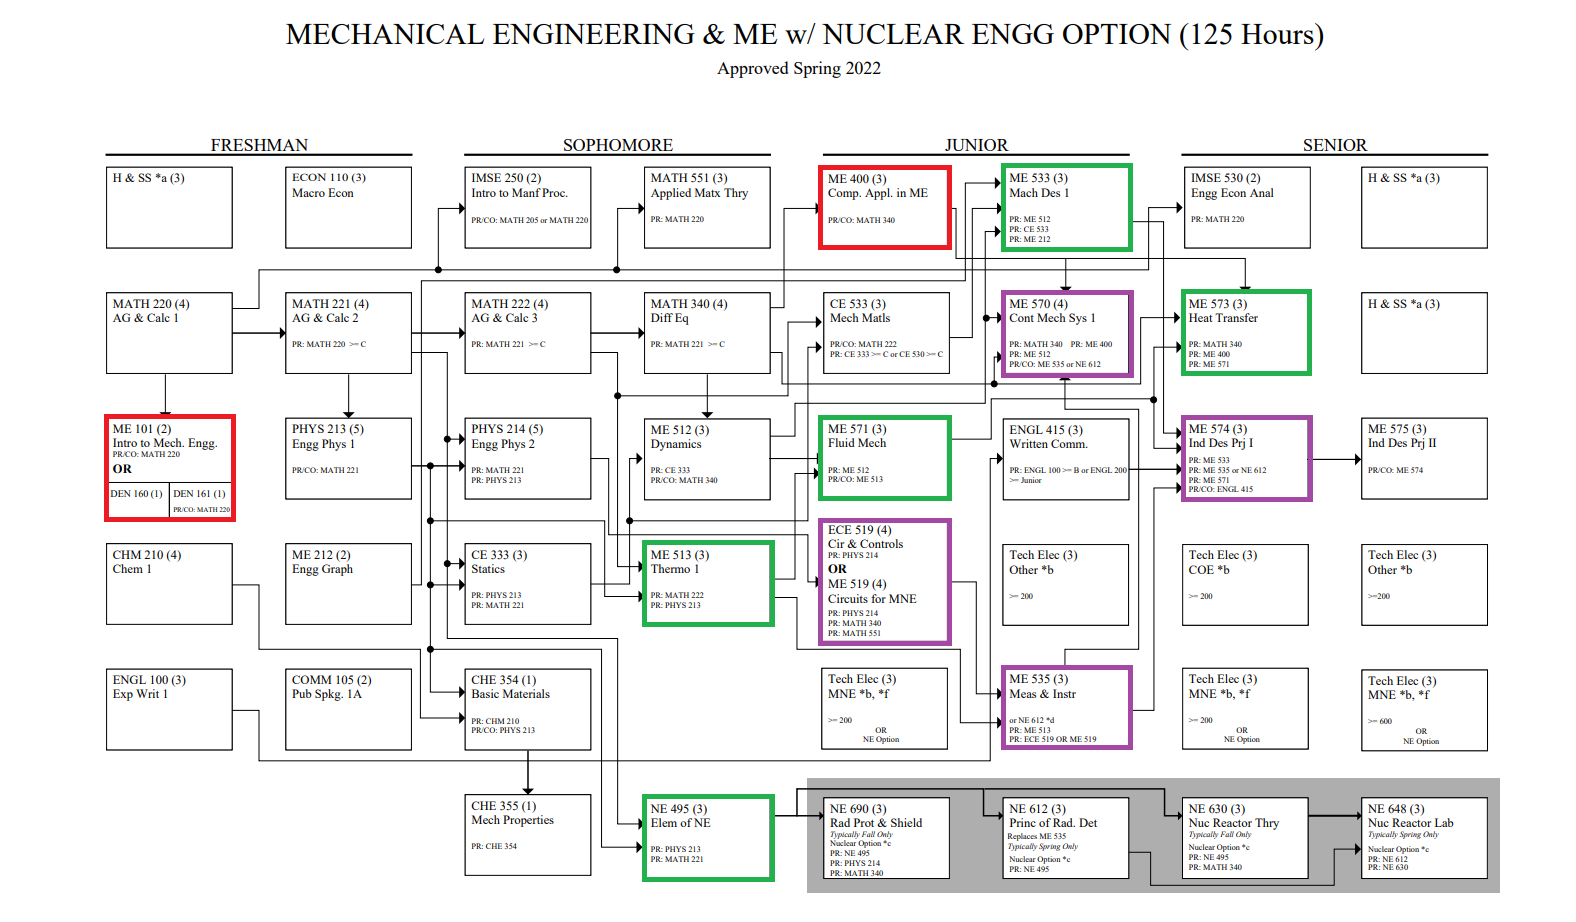
\includegraphics[width=\textwidth]{mne_flowchart}
    \begin{tabular}{l@{ : }l}
        Red & Teaches Programming \\
        Purple & Uses Programming \\
        Green & Does not utilize Programming, but could \\
    \end{tabular}
    \centering
    \caption{MNE Curriculum Flowchart}
    \centering
    \label{fig:mne_flowchart}
\end{figure}

The next class to use programming is also the only class dedicated to teaching programmig.
ME 400: Computer Applications in Mechanical Engineering begins with an introduction to C++
but then quickly moves to teaching embedded C++ for use on an ESP32. While the class
contains phenomenal material as it relates to embedded programming, its face paced nature
often leaves students confused on the fundamentals of programming. 

The next two classes to use programming are ME 519: Cirucuits for MNE and ME 400:
Control of Mechanical Systems 1. Both classes use MATLAB for system analysis and only use
MATLAB's introductory Onramp to teach students how to use the language and environment.
Due the inadequate foundations in programming, many students struggle with the new language,
making it difficult for them to understand the new concepts being taught, such as a PID
controller.

The last, non-project based class to use programming is ME 535: Measurements and Instrumentation.
This class is a bit of an outlier, because it uses the graphical programming language known
as LabVIEW. Rather than writing lines of code, users can add and edit ``blocks'' that have
predefined functionality. The class teaches how to use every block that is needed to complete
the labs, but much of the details are left unexplored.

The final class that utilizes programming is ME 574: Interdisciplinary Design Project 1, 
better known as Senior Design 1. This class revolves around the completion and fabrication
of a single product. This product always has some electromechanical aspects that need to
be controlled by a microcontroller. Neither the device not language used is moderated by
the class instructors.

As it currently stands, the MNE department makes use of four different programming languages
in required classes: C++, MATLAB, Python, and LabVIEW. While each of these languages and 
environments come with their own benefits, and there is certainly a benefit to using 
multiple languages, many students find themselves confused by the variety. Rather than
feeling confident in one language, they feel unconfident in four languages.

In addition to the weak foundation and lack of consistency, many classes are not using
programming that would benefit from using it. Any class that uses tables to look up values
or iterative design methods, such as Thermodynamics, Heat Transfer, or Fluid Mechanics, 
would make good use of programming. 

Based on experience as an instructor of ME 570 and ME 574 for the better part of 
four years, the majority of students struggle with using MATLAB and C++. This makes it 
difficult for students to learn how to design a control system when they do not understand 
the tool they are using to analyze it.

\section{Scope of Work}

While the motivation for this work relies on the idea that a more consistent approach to
learning and applying programming would benefit students and improve their problem solving
abilities, this project does not seek to prove or verify this claim. Neither does this
work set out to prove that the proposed solution is the best solution for the assumed
problem. This project merely seeks to identify a potential path forward while 
demonstrating both the advantages and disadvantages of the curriculum. 

This work will take time to point out benefits and drawbacks compared to the current 
curriculum, but given that no other possible solution is considered, it would be
premature to draw conclusions relating to the ``best'' path forward. However, there 
will be a brief discussion of alternative options in the concluding chapter of the paper.

\section{Structure of Work}

Since this body of work does not set out to prove a hypothesis, opting instead to demonstrate
a consistent usage and application of programming across the MNE curriculum, the format of
this paper will be adjusted accordingly. The next chapter, titled ``A Cohesive Programming
Curriculum,'' will discuss the foundation of the new implementation, such as the language,
hardware, and development environment. It will also discuss the general goal of the changes.

Subsequent chapters will each be dedicated to a class in the MNE curriculum. These chapters
will give a course overview, describe the new or altered assignments, and give a list
of deliverables for that course. The actual assignment descriptions and implementations
are not contained in the chapters themselves but rather in a repository on GitHub. Each 
chapter will have a folder of the same name dedicated to it in the repository. This folder
will contain everything an instructor would need to assign and grade the new assignments.


    \chapter{A Cohesive Programming Curriculum}
    \section{Curriculum Proposal}

The primary concerns addressed in Chapter 1 are as follows:

\begin{enumerate}
    \item Students lack a solid foundation in the fundamentals of programming.
    \item Programming is under utilized as a method of problem solving.
\end{enumerate}
To address the first issue, this paper would like to make two proposals: the adoption of a single programming 
language and the restructuring of electronics classes in the department. First, the goal of adopting a single 
programming language is to give students a more thorough understanding in a single language rather than 
a shallow understanding of four languages. The language chosen in this project is Python. In conjunction with 
Python, a consistent environemnt should be used as well. A consistent environment will prevent unnecessary 
confusions from IDE specific features and setup requirements. The choosen environment for this project is 
Visual Studio Code. To replace the work done on the Arduino Uno and ESP32, a Raspberry Pi Pico will used 
thanks to its seemless integration with both Python and Visual Studio Code. For more details regarding these 
choices, see Sections 2.2-2.5.

Second, the goal of restructuring electronics classes is to give students a dedicated ``fundamentals of 
programming'' class rather than a microcontroller class that teaches programming out of necessity. This
change, however, will not be addressed for the bulk of this work. Significant changes to the courses
required in the curriculum are difficult to pass, and always come with trade-offs. As such, discussion of 
this topic will be saved for reflection in the conclusion of this paper.

To address the second primary concern, the under-utilization of programming in the curriculum, two more
changes are being proposed: the addition of assignments or projects that make use of programming software
and the creation of a MNE library for use in most, if not all, MNE classes. The majority of this paper, as
well as the supporting repository, is dedicated to creating assignments that utilize programming for classes
that do not have one, translating assignments from other languages in classes that do utilize programming,
and creating a functional, though incomplete, Python package that could be used throughout the department.
The goal of these changes is twofold: teaching students how to use modern problem solving techniques to find 
solutions and giving students a chance to reinforce the programming skills they were taught. By giving
students a more consistent approach to programming, as well as more use cases for the value of programming,
students will become more confident and more capable as problem solvers and engineers.

Through the course of this project, many different Python packages and Visual Studio Code extensions will
be utilized. Thankfully, the installation and usage steps are simple, and can be combined into a single 
step in both cases. The Visual Studio Code extensions can all by downloaded at once using an
extension pack called KSU Mechancial Engineering Extension Pack. The necessary Python packages can also
all be installed at once from a requirements file. In some cases, it may be preferable to use Anaconda,
a Python distribution that comes many standard packages, to prevent the need for students to install
packages on their own. To see a full list of the applications, packages, and extensions and their versions, 
see Appendix \ref{appendix:appendix_versions}. For installation instructions, see the git repository in 
Appendix \ref{appendix:appendix_github}. 

\section{Python}

Python is a multipurpose, interpreted programming langauge that emphasises code readability. The langauge is
was originally introduced by Guido van Rossum in 1991 and has gone through three major versions,
the most recent being the aptly named Python 3. Using Python, particularly for first time programmers,
comes with the following benefits:

\begin{itemize}
    \item Python is an interpreted language; therefore, users do not need to install and configure
    a compiler. The setup process for a compiler can often be confusing and a major barrier to entry
    for new users. Since Python does not have a compiler, the only download that is necessary to run 
    a .py file is Python itself. The lack of a compiler does come with some downsides, namely speed,
    but these will be addressed later on.
    \item Python is designed to be human readable. This means that the syntax of the language closely
    matches the structure of the plain English. This emphasis on readability greatly reduces the
    burden on new users and bolsters code comprehension, even in more experienced coders. Consider 
    a program that prints the phrase "Hello world!"  to the terminal. In C++, this would be done with 
    the following code:

    \begin{lstlisting}[language=C++]
    #include <iostream>

    int main() {
        std::cout << "Hello world!" << std::endl;
        return 0;
    }
    \end{lstlisting}

    Not only is this code not human readable, but it requires the use of imports, functions, return
    values, namespaces, and non-obvious syntax. In Python, however, only one line of code is needed:

    \begin{lstlisting}[language=Python]
    print("Hello world!")
    \end{lstlisting}
    \item Python is a multipurpose, general-use language. The language is adept at everything from
    data science to building a webiste to powering a microcontroller (using MicroPython). With such 
    a wide breadth of use cases, learning the language opens the door to countless different applications 
    and projects.
    \item Python is open-source and currently one of the most used languages. Thanks to its popularity,
    many tools exist to make programming with Python easier, more powerful, and more accessible such
    as integrations with Jupyter Notebooks and Visual Studio Code. However, this can potentially be 
    two edged sword, as will be discussed later.
    \item Python has an easy to use package manager called pip, which is a recursize acronym for pip
    installs packages. This package manager makes it incredibly easy to both install and use non-standard
    libraries in Python.
\end{itemize}

Python provides a solid starting point for new programmers while also being fully capable of high-level,
advanced programming making it a good language for users of all skill levels. However, it does not come 
without concerns of its own, most noteably version controlling. This will be addressed at
length in a future chapter.

\section{MicroPython}

MicroPython is a slimmed version of Python that is designed to run on microcontrollers, such as the
Raspberry Pi Pico or ESP32. This Python derivative removes some high level features in exchange for
a smaller interpreter and a machine library dedicated to interacting with the hardware of the 
microcontroller, which Python would normally not interact with.

While MicroPython comes with all the benefits of Python, it also comes with one of the drawbacks
of Python: speed. Unlike traditional low level languages like C/C++, MicroPython is not compiled,
making it significantly slower than comparable languages. In some applications, the difference in
speed has no affect on the application. Others, like a control system, heavily depend on fast loop
times and are greatly impacted by speed.

\section{Raspberry Pi Pico}

The Raspberry Pi Pico is a small-but-powerful microcontroller made by Raspberry Pi. A microcontroller
is an electronic input-output device capable of running uploaded code. It is differentiated
from a microprocessor, such as a Raspberry Pi 5 or a desktop computer, by the fact that it does not run 
an operating system. 

The using a Pico, as a newer competitor in the saturated microcontroller market, begs the question of 
``why not use the Arduino Uno or ESP32?'' While all three devices support ADC, SPI, I2C, and have 
around 40 GPIO pins, only the ESP32 and Pico support MicroPython, as well as built in wireless and 
Bluetooth connectivity.

A case could be made for using the ESP32 over the Pico, given its rise in popularity in the home
automation space. However, the ESP32 comes with greater restrictions in GPIO usage and the majority
of its documentation and drivers are for C++ programs rather than MicroPython, giving the Pico an
edge in user friendlinesss.

As was the case with Python and MicroPython, the Pico does not come without drawbacks. Almost all 
sensors come with drivers written in C++ for the Arduino Uno or ESP32. This is not the case for 
the Pico. Some sensors made specifically to work with the Pico come with drivers, and others may 
be found on GitHub thanks to the work of another tinkering user, but many pieces of hardware do 
not have driver support for the Pico. This could end up being a limiting factor for students trying 
to do unguided projects.

\section{Visual Studio Code}

Visual Studio Code is a cross-platform, highly customizeable development environment created by
Microsoft. It is one of the most used and most accessible development environments available, 
and supports use with any language. VSCode can almost be thought of as a Word processor where 
spell check looks for syntax errors and keywords instead of grammatical mistakes. By installing
extensions, which can be done from inside VSCode, developers can write code for nearly any 
microcontroller or processor and in nearly any language.

For the purposes of the Mechanical Engineering Department, extensions for Python, MicroPython and
the Pico, and Jupyter Notebooks (a type of interactive programming environment that will be utilized
later) will be used. The extensions are both easy to use and install, but share a downside with
Python: version control. Since these extensions are always in active development and get updated
to work with the newest version of Python and Visual Studio Code, which may not always be desireable.
This issue will be discussed in greater detail in a later chapter.

    
    \chapter{DEN 161: Engineering Problem Solving}
    \section{Course Overview}

DEN 161: Engineering Problem Solving is a lab-style course that complements the lecture-oriented DEN 160: 
Engineering Orientation. The class focuses on providing hands-on, problem-solving experiences through projects 
from multiple engineering disciplines. While these projects serve as the students' introduction to different 
engineering disciplines, they also develop the core tools needed to be a successful engineer. 

The current iteration of DEN 161 has three sections of interest to this body of work: data analysis using 
Microsoft Excel, data analysis using Python, and embedded programming using an Arduino Uno.

Microsoft Excel is used to introduce the concept of data analysis to students. Students are tasked with 
manipulating data and finding different statistical properties of given data. This proves to be an effective 
point of entry given to data analysis since many students are familiar with Microsoft Excel or Google Sheets.

Python is then introduced as an alternative method of solving the same problems. The lectures and assignments 
focus on data calculations to verify designs and general code inspection to understand how the program works. 
These lectures are done using Jupyter Notebook in Anaconda's Spyder IDE. 

Following the introduction to Python, a Stoplight Activity is assigned. This project introduces students to 
circuitry and microcontrollers through the creation of a stoplight using 3 LEDs and an Arduino Uno. The Arduino 
Uno is programmed using C++ in the Arduino IDE.

\section{Project Redesign}

Thanks to the solid programming core created by the instructors, the proposed changes are minor, and result in 
few changes to the current curriculum. Two changes are proposed: the adoption of Visual Studio Code as a 
development environment and the migration from Arduino Unos to Raspberry Pi Picos. 

The class currently uses an IDE by the name of Spyder. Spyder is a popular IDE for data science applications and 
has the to ability to seamlessly integrate with Jupyter Notebooks. However, Spyder does not have the ability to work 
with a MicroPython device, such as the RPi Pico. Visual Studio Code, on the other hand, has an extension that 
integrates Pico controls directly into the interface, making it a one-stop-shop for both the data analysis and 
embedded systems development in DEN 161. Visual Studio Code also has Jupyter Notebook extensions that allow for 
a first class experience.

The second proposed change is transitioning from the Arduino Uno to a Raspberry Pi Pico. The reason for this 
change is twofold. First, the Pico can run using MicroPython, a lightweight implementation of Python, which has 
the same syntax as Python. This allows students to focus on understanding one language, Python, rather than 
learning both Python and C++. Switching to the Pico also opens the door to using a single development environment. 
While the Arduino can be programmed using Visual Studio Code, the setup process is non-trivial, and requires a 
strong understanding of the operating and file system of the computer. 

With these changes in mind, the first two assignments created serve as a segue from using Excel for data analysis to 
using Python. The first of the two, Assignment \ref{engg_prob_solve_assignment_1}, requires students to convert 
tire rpm data to speed data, find several statistical properties of the data, and then plot it. The assignment
is done in class both in Excel and Python to showcase the differences.

\assignments{DEN 161: Assignment 1}
\label{engg_prob_solve_assignment_1}

\begin{tcolorbox}[breakable, enhanced jigsaw, title=DEN 161: Assignment \ref{engg_prob_solve_assignment_1}, 
    colframe=ksu-purple, colback=ksu-gray]

    \textbf{Problem Statement}
    \parindent15pt

    You are given data for the tire rotations per minute in a file called `tire\_rpm.csv' and are tasked with 
    finding the max, min, mean, mode, and median speed of the vehicle. Bonus points for a graph!

    \tcblower
    \textbf{Problem Solution}
    \parindent15pt

    For the full solution, see Appendix \ref{appendix:appendix_github}. The following shows the process
    of reading information from a .csv file.
    
    To solve this problem, let's split it into steps and address the issues one at a time.

    \begin{enumerate}
        \item Read and parse the data from the .csv file
        \item Convert the RPM data into vehicle speed 
        \item Find the max, min, mean, mode, and median
    \end{enumerate}
    
    \noindent \textbf{Step 1: Read and parse the data}
    
    To begin, we will import the built-in csv library. This Python package makes it easy to parse data from csv 
    files, and takes away the burden of writing code to split the data. We will also import the math library.

\begin{python}
import csv
import math
\end{python}

    We will start by creating an empty list for our rpm values to be stored in. Next we will open the .csv 
    file and read it.

\begin{python}
with open("tire_rpm_example.csv", "r") as file_contents:
csv_reader = csv.reader(file_contents,delimiter=",")
rpm = []
for rpm_row in csv_reader:
    for rpm_value in rpm_row:
        rpm.append(int(rpm_value))
print(f"Tire RPM: {rpm}")
\end{python}
\end{tcolorbox}

After completing the in-class example, a similar assignment is given for homework, as shown in Assignment
\ref{engg_prob_solve_assignment_2}. Rather than writing the code from scratch, students must make several 
changes and add comments to the file.

\assignments{DEN 161: Assignment 2}
\label{engg_prob_solve_assignment_2}

\begin{tcolorbox}[breakable, enhanced jigsaw, title=DEN 161: Assignment \ref{engg_prob_solve_assignment_2}, 
    colframe=ksu-purple, colback=ksu-gray]

    \textbf{Problem Statement}
    \parindent15pt

    Make the following changes to the given Python file:

    \begin{enumerate}
        \item Change the input file to the homework data set.
        \item Change the tire diameter to utilize user input.
        \item Change the print statements to have 0 decimal places.
        \item Anywhere there is a \#COMMENT, leave a comment explaining what the following lines of code do.
    \end{enumerate}
               
    Optionally, complete the bonus assignment question at the bottom of the file.
    

    \tcblower
    \textbf{Problem Solution}
    \parindent15pt

    For the full solution, see Appendix \ref{appendix:appendix_github}. The following shows the changed file
    name, user input, and descriptive comments.

\begin{python}
# Import statements to make library methods 
# available in this file
import csv
import math
import statistics
from matplotlib import pyplot

# Open and read data from a csv file into Python
with open("tire_rpm_homework.csv","r", 
          encoding="utf-8") as file_contents:
    csv_reader = csv.reader(file_contents,delimiter=",")
    rpm = []
    for rpm_value in next(csv_reader):
        # Turn the rpm_value (which would be a string) 
        # into an integer and add it to a list of rpms
        rpm.append(int(rpm_value))

# Ask the user to input the tire diameter
tire_diameter = input("What is the tire diameter?")
\end{python}
\end{tcolorbox}

The third assignment, shown in Assignment \ref{engg_prob_solve_assignment_3} was translated from the 
current Stoplight project used in the class \cite{stoplight}. An example file
demonstrating how to operate the LEDs serves as the starting point for the project. To complete the
assignment, students need to rearrange the \pyth{pin.high()} calls and change the sleep timings.

\assignments{DEN 161: Assignment 3}
\label{engg_prob_solve_assignment_3}

\begin{tcolorbox}[breakable, enhanced jigsaw, title=DEN 161: Assignment \ref{engg_prob_solve_assignment_3}, 
    colframe=ksu-purple, colback=ksu-gray]

    \textbf{Problem Statement}
    \parindent15pt

    Using the Raspberry Pi Pico and three LEDs given out in class, write a program that will operate
    the LEDs like a stoplight. For bonus assignment credit, write a program that will blink SOS in Morse code.
    
    \tcblower
    \textbf{Problem Solution}
    \parindent15pt
    
    For the full bonus assignment solution and the example file, see Appendix \ref{appendix:appendix_github}. 
    The following shows the entire solution to the stoplight portion of the assignment.

\begin{python}
from machine import Pin
import time

# Declare the pins and the pin mode
red_led = Pin(18, Pin.OUT)
yellow_led = Pin(17, Pin.OUT)
green_led = Pin(16, Pin.OUT)

# Begin looping phase
while True:
    # Turn on the red led for 5 seconds
    green_led.low()
    yellow_led.low()
    red_led.high()
    time.sleep(5)

    # Turn green led on and red led off for 5 seconds
    green_led.high()
    red_led.low()
    time.sleep(5)

    # Turn yellow led on and green led off for 2 seconds
    yellow_led.high()
    green_led.low()
    time.sleep(2)
    \end{python}
\end{tcolorbox}

The proposed changes aim to increase student understanding by reducing the number of systems they are introduced 
to. Instead of two languages and two editors, students will only need to learn one language in one editor. The 
work done by these projects directly correlates with ABET Student Outcomes 6 and 7 and weakly correlates with 
Outcomes 1 and 3, as seen in Appendix~\ref{appendix:appendix_abet}.

\section{Project Redesign Assessment}

The project proposal for DEN 161 is unique from the other classes in this work because the proposed changes were
implemented into the standard class curriculum. The second week of Python was replaced with the tire RPM problem
and the Arduino Uno was replaced by the Raspberry Pi Pico in the stoplight project. The adoption was largely 
successful, and the instructors felt that it was a step in the correct direction. That is not to say that there
were no pain points.

The biggest hindrance encountered in the Fall 2023 was general file system comprehension. Many students did not 
know where downloaded files go or how the file system (both File Explorer and Finder) were structured. This proved 
to be an issue for both the tire RPM question and the stoplight example. For Python to locate the .csv file 
with the RPM data, either the full path to the file needs to be provided, relative to the current working directory,
or the file needed to be in the same folder as the script. To get the MicroPico extension to work correctly in
Visual Studio Code, a working directory needs to be set. 

Both of these issues can likely be solved with the same two methods. First, time will be spent in a previous lecture
to talk about the file system. This is basic information that is required to effectively use a computer. Second,
files for assignments will be distributed in zip files. This will nearly guarantee that files have the correct
relative location. This will introduce a new issue of trying to link and edit files in a zip folder, but hopefully
it is an easier fix than trying to hunt down files on student's laptops.

The Fall 2023 semester also found that using Visual Studio Code for both the data analysis and Pico portions of the
class is better for students than using Spyder for the data analysis and VSCode for the Pico. 

An additional pre-class assignment will also be created that will require students to verify that they have
done the necessary installations before coming to class. Though this is not an issue directly caused by the changes
made, it did directly inhibit student learning.

The final issue, and perhaps the most concerning, is the unreliability of the MicroPico extension when not used 
exactly as intended. While no connection issues ever occurred during testing, a non-trivial number of students
experienced issues with the MicroPico extension. Since no issues have been encountered by the instructors at this
point, it is hard to pinpoint the exact cause. Fixes for different issues can be found in the 
``usage-and-installation'' folder in the GitHub Repository.

\section{Recommendations for Course Integration}

After completing the new (and translated) assignments in DEN 161, students should be able to identify the components 
used in simple programs and explain the functionality of code blocks. With this understanding, students should also 
be able to use simple programming techniques to alter the functionality of existing code. 

To achieve these outcomes, DEN 161 should continue teaching its introduction to Python as well as continue
using the adopted material presented above. In response to the first semester assessment, Visual Studio
Code should be adopted over Spyder for the Python assignments, and files should be distributed through
the use of zip files to prevent issues with file location. To contend with the issues caused by the lack
of file system knowledge, as well as to preemptively address the issues with extracting zip files, additional
class time should be spent ensuring students understand the basics of a file system. This ability to use
a file system extends far past programming and is essential for every student.

\section{Project Deliverables}

In the GitHub repository associated with this paper, which can be found in Appendix \ref{appendix:appendix_github},
the folder titled ``3-engineering-problem-solving,'' there are several folders containing different problems and 
examples. The folder also contains a README that details what is in each file and what software is needed to 
complete the assignments. 

The first folder is a tire RPM example problem that is to be completed in class, after having completed the Excel
lectures and the introduction to Python lectures. This will show students the benefits of using a
language like Python over Excel. To go along with the example problem is a similar tire RPM homework assignment.
The code needed to complete the assignment is all provided to students, with a handful of tasks left up to them,
as detailed in the homework file. 

Finally, the stoplight folder contains the starter code to give students for the stoplight assignment, a solution
key, and a file demonstrating Morse code on the Pico. Installation instructions for the using the Pico can be found
in the ``usage-and-installation'' folder in the repository.


    \chapter{ME 513: Thermodynamics}
    \section{Course Overview}

ME 513: Thermodynamics is a lecture based class that focuses on the interplay of heat, work, and energy in both
open and closed loop systems. While there is no lab portion to the class, significant lecture time is spent
solving problems and working examples, and a new homework is assigned every lecture to give students a chance
to apply the new concepts taught that day.

Most problems in thermodynamics follow a similar solution path. First, students must recognize the different
states in the system. Once the different states are identified, the values for temperature, power, energy,
entropy, etc. must be found for each state. The exact values needed, and retrievable, vary depending on the
given system. This process is known as setting the state. Once the state has been set, known laws of
thermodynamics can be applied and the question can be solved.

For most questions, the majority of time is spent setting the state. This involves using known properties, 
usually given in the problem statement, to look up values in property tables in a thermodynamics textbook. 
This often proves to be a very time-consuming process, especially when interpolation is required to get 
property values. And once iteration is introduced, such as in a design problem, manually searching through
tables becomes impractical, if not impossible. This is where the use of a programming language would become 
highly beneficial.

Thermodynamics, as it currently stands, make no use of programming to complete assignments.
This can be attributed to ME 513 coming prior to ME 400, the only programming class in the 
curriculum. However, with the recent programming additions made to DEN 161, students have been introduced
to programming and, with the help of an example, should be capable of solving these questions as a small
project or assignment.

\section{New Assignments}

Since no assignments currently make use of programming, two new assignments have been adapted from 
\textit{Fundamentals of Engineering Thermodynamics, 9th Edition} \cite{thermodynamics} to demonstrate
how programming could be beneficial to the course. Both assignments will make use of a Python library called
$PYroMat$ \cite{chris_martin_2022_7262173}, a free, open source library dedicated to making thermodynamic properties 
readily available. They will also both make use of Jupyter Notebooks for cleanly presenting questions, 
commentaries, and code while solving the question.

The first assignment, Assignment \ref{thermo_assignment_1}, is a five state system that does not require 
iteration or plotting. This example follows the structure of a typical question in thermodynamics. The student 
must identify the states, list the known properties for each state, and then either search for additional 
values in a table or calculate them with known values. After this, the laws of thermodynamics are applied, 
equations are balanced, and the questions solved.

\assignments{ME 513: Assignment 1}
\label{thermo_assignment_1}

\begin{tcolorbox}[breakable, enhanced jigsaw, title=ME 513: Assignment \ref{thermo_assignment_1}, 
    colframe=ksu-purple, colback=ksu-gray]

    \textbf{Problem Statement}
    \parindent15pt

    Water is the working fluid in a Rankine cycle. Steam exits the steam generator at 1500 
    lbf/in\textsuperscript{2}  and 1100°F. Due to heat transfer and frictional effects in 
    the line connecting the steam generator and turbine, the pressure and temperature at the 
    turbine inlet are reduced to 1400 lbf/in\textsuperscript{2} and 1000°F, respectively. Both the 
    turbine and pump have isentropic efficiencies of 85\%. Pressure at the condenser inlet 
    is 2 lbf/in\textsuperscript{2}, but due to frictional effects the condensate exits the 
    condenser at a pressure of 1.5 lbf/in\textsuperscript{2} and a temperature of 110°F. The 
    condensate is pumped to 1600 lbf/in\textsuperscript{2} before entering the steam generator. 
    The net power output of the cycle is 1x10\textsuperscript{9} Btu/h. Cooling water experiences 
    a temperature increase from 60°F to 76°F, with negligible pressure drop, as it passes 
    through the condenser. Determine for the cycle:

    \begin{enumerate}
        \item the mass flow rate of steam, in lb/h.
        \item the rate of heat transfer, in Btu/h, to the working fluid passing through the steam 
        generator. 
        \item the thermal efficiency.
        \item the mass flow rate of cooling water, in lb/h.
    \end{enumerate}

    Be sure to leave specify all assumptions and comment on the functionality of the code. 
    To access the thermodynamic tables for water, import $PYroMat$ using the cell below.

    \tcblower
    \textbf{Problem Solution}
    \parindent15pt

    For the full solution, see Appendix \ref{appendix:appendix_github}. Below is an example of 
    importing $PYroMat$, setting the correct units, and creating an object for a specific
    substance.

\begin{python}
import pyromat

pyromat.config["unit_energy"] = "BTU"
pyromat.config["unit_force"] = "lbf"
pyromat.config["unit_mass"] = "lb"
pyromat.config["unit_temperature"] = "F"
H2O = pyromat.get("mp.H2O")
\end{python}

To find specific property data, such as enthalpy and entropy, call the appropriate method
on the substance object, H2O in this case, and pass the temperature and pressure.

\begin{python}
# State 1
p1 = 1400 # lbf/in^2
T1 = 1000 # deg F
h1 = H2O.h(T=T1, p=p1) # Btu/lb
s1 = H2O.s(T=T1, p=p1) # Btu/(lb*F)
\end{python}
\end{tcolorbox}

The second assignment, Assignment \ref{thermo_assignment_2}, better showcases the benefits of 
programming. This question uses both iteration and plotting to show the changes in quality 
and thermal efficiency as the pressure increases. If done by hand, this would be a difficult 
and tedious task. But when programming, it only requires a few extra lines of code.

\assignments{ME 513: Assignment 2}
\label{thermo_assignment_2}

\begin{tcolorbox}[breakable, enhanced jigsaw, title=ME 513: Assignment \ref{thermo_assignment_2}, 
    colframe=ksu-purple, colback=ksu-gray]

    \textbf{Problem Statement}
    \parindent15pt

    Steam heated at constant pressure in a steam generator enters the first stage of a
    supercritical reheat cycle at 28 MPa, 520°C. Steam exiting the first-stage turbine at 6 MPa is
    reheated at constant pressure to 500°C. Each turbine stage has an isentropic efficiency of 78\%
    while the pump has an isentropic efficiency of 82\%. Saturated liquid exits the condenser that
    operates at constant pressure, p.

    \begin{enumerate}
        \item For p = 6 kPa, determine the quality of the steam exiting the second stage of the 
        turbine and the thermal efficiency.
        \item Plot the quantities of part (1) versus p ranging from 4 kPa to 70 kPa.
    \end{enumerate}

    Be sure to leave specify all assumptions and comment on the functionality of the code. 

    \tcblower
    \textbf{Problem Solution}
    \parindent15pt

    For the full solution, see Appendix \ref{appendix:appendix_github}. Below is an example of 
    iterating through varying pressure values to create a list of quality values.

\begin{python}
p_list = [x * 10**(-3) for x in range(4, 71)]
x_list = []
n_list = []

for p in p_list:
    # State 4
    p4 = p # MPa
    x4s = H2O.T(s=s3, p=p4, quality=True)[1]
    h4s = H2O.h(p=p4, x=x4s)
    h4 = h3 - nt2 * (h3 - h4s)

    # State 5
    p5 = p # MPa
    h5 = H2O.h(p=p5, x=0)
    v5 = H2O.v(p=p5, x=0)

    # State 6
    h6 = h5 + 1000 * v5 * (p6 - p5) / (np1)

    # Find the quality of the steam
    hf4 = H2O.h(p=p4, x=0)
    hfg4 = H2O.h(p=p4, x=1) - H2O.h(p=p4, x=0)
    x4 = (h4 - hf4) / hfg4
    x_list.append(x4)

    # Find the thermal efficiency of the cycle
    n = ((h1-h2)+(h3-h4)-(h6-h5))/((h1-h6)+(h3-h2))
    n_list.append(n)
\end{python}

    With the quality and pressures in hand, a graph can be generated with $matplotlib$.

\begin{python}
from matplotlib import pyplot as plt

plt.figure()
plt.plot(p_list, x_list)
plt.title("Quality vs Condenser Pressure")
plt.xlabel("Pressure (MPa)")
plt.ylabel("Quality (unitless)")
plt.show()
\end{python}
\begin{center}
    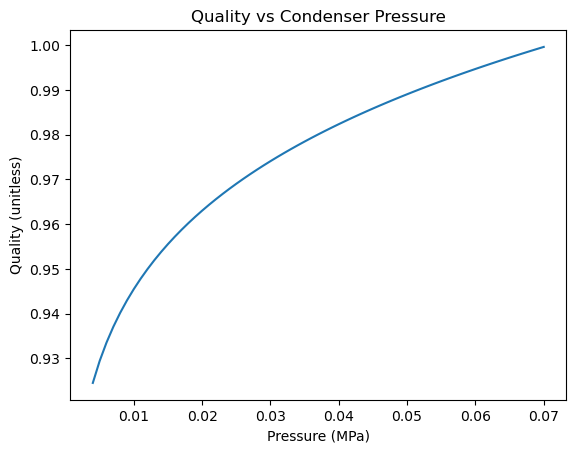
\includegraphics[width=\textwidth]{thermo_assignment_2.png}
\end{center}
\end{tcolorbox}

Using programming in this manner gives students a better idea of how real problems are solved by introducing
them to a more efficient and powerful solution method. These questions would also directly correlate to ABET 
Student Outcomes 1, 6, and 7 and weakly correlate to Outcome 3, as seen in Appendix \ref{appendix:appendix_abet}.

\section{Recommendations for Course Integration}

After completing the programming assignments in ME 513, students should be able to recognize when programming
techniques can be applied to solve a problem, explain how tools are used, and implement a program to solve 
a thermodynamics question. Of these objectives, an emphasis should be placed on the students' ability to apply
tools given by the instructor.

To accomplish this, ME 513 should adopt at least two required programming questions and add the option for 
students to continue using programming to solve homework questions. For example, the first assignment could
consist of a traditional by-hand solution with the second question being the same problem but with an additional
requirement of solving through programming. The second assignment could be a small project or a dedicated
programming assignment that requires graphing, iteration, or numerous table values. 

To supplement these assignments, at least
one lecture should be dedicated to showing how to solve a thermodynamics question with Python. In addition,
a ``cheat sheet'' of commands, library calls, and other necessary operations should be given to students.
By providing a sheet of code commands, students can focus on understanding and applying information.


\section{Project Deliverables}

In the GitHub repository associated with this paper, which can be found in Appendix \ref{appendix:appendix_github},
the folder titled ``4-thermodynamics'' contains both the problem statements and solution guides for the two questions
introduced in the previous section. The folder also contains a README that details what is in each file and 
what software is needed to complete the assignments. 

For these projects to be added to the class, the instructor would simply need to give the starting code to 
students as a problem statement. It may be beneficial to use Assignment 4.1 as an in-class example both to serve 
as a reminder of how to use Python with Jupyter Notebooks as well as a demonstration of how to use $PYroMat$ to 
access material properties and change property units.


    \chapter{NE 495: Elements of Nuclear Engineering}
    \section{Course Overview}

NE 495: Elements of Nuclear Engineering is a lecture based class that focuses on introducing
the fundamental concepts of chemistry and physics that form the field of nuclear engineering 
to mechanical engineering students. The class also serves as the sole entry point into the nuclear
program at K-State. 

As class with no lab section, homework assignments and tests make up the majority of the grade
for the class. Currently, the class also has one project where students use a geiger counter 
developed for the class to measure ionizing radiation. 

As is the case with ME 513: Thermodynamics, this class comes before ME 400 and, therefore, does
not utilize programming for any homework assignments or projects. With the changes to DEN 161,
and especially should changes come to other classes, such as ME 513, students should be able 
to solve these problems.

\section{New Assignments}

While no assignments currently make use of programming, many questions lend themselves nicely
to being solved with programming. This is thanks to the heavy reliance on tables and
constants used in solving NE problems. To demonstrate, three questions, one from an exam
and two from a homework, have been solved using Python with the help of a few open source
libraries: mendeleev, physdata, and scipy.

Unfortunately, no single library contains the full collection of properties to solve the range
of questions presented in NE 495. While inconvenient, this issue serves to highlight the 
importance of creating a package for the MNE department that consolidates and standardizes the
information and structure of property data. 

The first question, taken from the first exam in the class, is a Q-value question that uses 
the mendeleev library to pull element properties. The library contains information on the elements
and their isotopes that, once familiar, provide quick access to the mass and abundance values
needed to solve Q-value problems. Unfortunately, the library outputs a list of isotopes and 
has no method for retrieving a specific mass number. Because of this, a wrapper function was
written to allow for easy access to individual isotopes. This function mimics the work that
would be done in an MNE library.

The second and third questions are both taken from homework 20 and deal with photon interactions. 
These questions make use of the physdata library to get attenuation coefficients for different
molecules (water, in this example). Similar to mendeleev, this library does not have an easy, 
built-in method for getting this coefficient values at non-standard energy values. Once again, a
wrapper function was written to allow for easy access to interpolated values.

Using programming in this manner gives students a better idea of how real problems are solved by
introducing them to a more efficient and powerful solution method. These questions would also 
directly correlate to Abet Student Outcomes 1, 6, and 7, as seen in Appendix 
\ref{appendix:appendix_abet}. With the addition of a question that utilizes basic plotting, a 
weak correlation to Outcome 3 could also be added.

\section{Project Deliverables}

In the GitHub repository associated with this paper, which can be found in 
Appendix \ref{appendix:appendix_github}, the folder titled ``elements-of-nuclear-engineering''
contains both the problem statements and solution guides for the three questions introduced in 
the previous section. The folder also contains a README that details what is in each file and 
what software is needed to complete the assignments. 

For these projects to be added to the class, the instructor would simply need to give the 
skeleton files to students as a problem statement. It may be beneficial to use one of the questions 
as an in-class example both to serve as a reminder of how to use Python with Jupyter Notebooks 
as well as a demonstration of how to use the data libraries to access material properties.
    
    \chapter{ME 400: Computer Applications in Mechanical Engineering}
    \section{Course Overview}

ME 400: Computer Applications in Mechanical Engineering is a lecture based class with
one lab per week. The lectures initially emphasis learning the basic tools of
programming, looping, functions, classes, etc., while the remainder of the class
focuses on embedded programming and microcontroller hardware, which is the primary
objective of the class.

To complete labs, students use an ESP32, a powerful microcontroller made popular by
the home automation community, programmed with C++, an industry standard in embedded
applications. Since the class does not have any circuit prerequisites and does not 
teach, nor have the time to teach, circuit theory, the class instructors have created
PCBs that are plug-and-play for students to use. These custom PCBs are designed to have
the ESP32 as well as several other electronic components plug directly into it to
give them the ability to work together. Additional components include a small LCD 
touchscreen, buttons, LEDs, and buzzers. 

The labs in ME 400 take an iterative approach where subsequent labs will add features
and functionality on top of the previous week's lab assignment. This gives students
the experience of completing a relatively complex project without overwhelming them 
from the start. 

ME 400 serves as the primary introduction to programming in the mechanical department.
It is also the only class that spends significant teaching about programming and the
only class that gives instructions on microcontrollers. Unfortunately, the class comes
late in the curriculum, after many classes that would benefit from using programming,
and focuses the majority of its time on embedded programming, often to the detriment
of a fundamental understanding of programming. This is a topic of much debate, and
will be addressed in the concluding chapters.

\section{Project Redesign}

Since ME 400 is a programming course, no new assignments are being created for this
project. Instead, a pre-existing lab has been translated from C++ on the ESP32 to
MicroPython on the Raspberry Pi Pico. The translated lab exercise, partially shown in 
Assignment \ref{comp_app_assignment_1}, is the concluding
assignment in a string of lab exercises dedicated to programming the game "Simon Says"
\cite{simon-says}.

The goal of the exercise is to create a replayable, memory-based game that imitates the
children's game Simon Says. To do this, students have to use the LCD screen, five 
buttons, four LEDs, a buzzer, and an IR remote. The lab exercise chosen aims to 
demonstrate how the Pico and MicroPython can handle the same projects and electronics 
that the ESP32 and C++ can. 

\assignments{ME 400: Assignment 1}
\label{comp_app_assignment_1}

\begin{tcolorbox}[breakable, enhanced jigsaw, title=ME 400: Assignment \ref{comp_app_assignment_1}, 
    colframe=ksu-purple, colback=ksu-gray]
    \textbf{Problem Statement}
    \parindent15pt

    For the full problem statement, please see Appendix \ref{appendix:appendix_github}.
    Complete each of the following steps. When you have completed all steps assigned, upload the
    files associated with the exercise on Canvas. Make sure the filenames you upload as part of
    your exercise submission have the exact names specified in each steps of this exercise. If the
    filenames do not match exactly, then your submission will not be graded.

    \medskip
    \noindent \textbf{Background}

    Simon is an electronic game of short-term memory skill invented by Ralph H. Baer and Howard J.
    Morrison and programmed by Lenny Cope. The game is implemented using a combination of hardware
    and software, and the physical interface consists of four quadrants as shown in Figure 1.

    When the game starts, a random sequence is presented to the user by lighting the associated
    quadrants and playing a tone that is specific to each quadrant. Then the user is required to repeat the
    sequence. If the user succeeds, then the series becomes progressively longer and more complex.
    Once the user fails to enter the correct sequence, the game is over.

    A simple version of this game will be implemented as part of this exercise. This task will test your
    understanding of incorporating and writing functions, passing arguments to functions, implementing
    logic in loops, implementing branching logic, and working with arrays.

    \medskip
    \noindent \textbf{Submission}

    Upload the files exercise\_07.py to Canvas once the exercise has been completed. The code will
    be evaluated as follows:

    \begin{enumerate}
        \item It will be evaluated to make sure the proper coding techniques were used to implement the
        associated functionality.
        \item It will be evaluated to ensure the associated code runs successfully.
        \item It will be evaluated to ensure the associated code returns accurate and complete results.
        \item It will be evaluated to ensure that the correct file names specified for each problem were
        uploaded to Canvas.
        \item It will be evaluated to make sure the implementation uses correct indentation.
        \item It will be evaluated to determine if suitable comments have been included.
    \end{enumerate}

    \tcblower
    \textbf{Problem Solution}
    \parindent15pt

    For the full solution, see Appendix \ref{appendix:appendix_github}. Below is an example of 
    importing the drivers and creating objects for each piece of hardware used.

\begin{python}
import time
from random import randrange, seed
from machine import Pin, PWM, SPI

from ir_remote_driver import IRRemote
from lcd_display_driver import Display, color565, XglcdFont
\end{python}

The infrared remote will be attached to GPIO pin 15 and set as an input.

\begin{python}
ir_remote = IRRemote(Pin(15, Pin.IN))
\end{python}

The piezo buzzer will be attached to pin 9 and will use pulse width modulation. The 
\pyth{buzzer_tones} list contains the pitches for the buzzer to play.

\begin{python}
buzzer = PWM(Pin(9))
buzzer_tones = [131, 165, 196, 262]
\end{python}

Next, the display needs to be attached using an SPI connection.

\begin{python}
spi = SPI(
    0, 
    baudrate=10000000, 
    polarity=1,
    phase=1,
    bits=8,
    firstbit=SPI.MSB,
    sck=Pin(18), 
    mosi=Pin(19),
    miso=Pin(16)
)
display = Display(
    spi, dc=Pin(20), cs=Pin(17), rst=Pin(21))
display.clear()
\end{python}

Finally, a font to use for any printed text to the display must be added.

\begin{python}
espresso_dolce = XglcdFont(
    'fonts/EspressoDolce18x24.c', 18, 24)
\end{python}
\end{tcolorbox}

To use the LCD screen and the IR remote, drivers needed to be created for the Pico. 
The drivers provided in the repository are modified versions of
rdagger's micropython-ili9341 library \cite{micropython-ili9341} and Peter Hinch's 
micropython\_ir library \cite{micropython_ir2020}. The modified drivers would be given to 
students, and they would not be expected to modify them in any way.

As previously mentioned, the class uses several custom PCBs to facilitate the use
of different circuit components. However, no circuit board was designed for this 
project, so the wiring was done by hand, as seen in Figure \ref{fig:simon_says}. Only 
small changes to hole locations and traces would be needed to adapt the current PCBs 
into a useable form for the Pico.

\begin{figure}[h]
    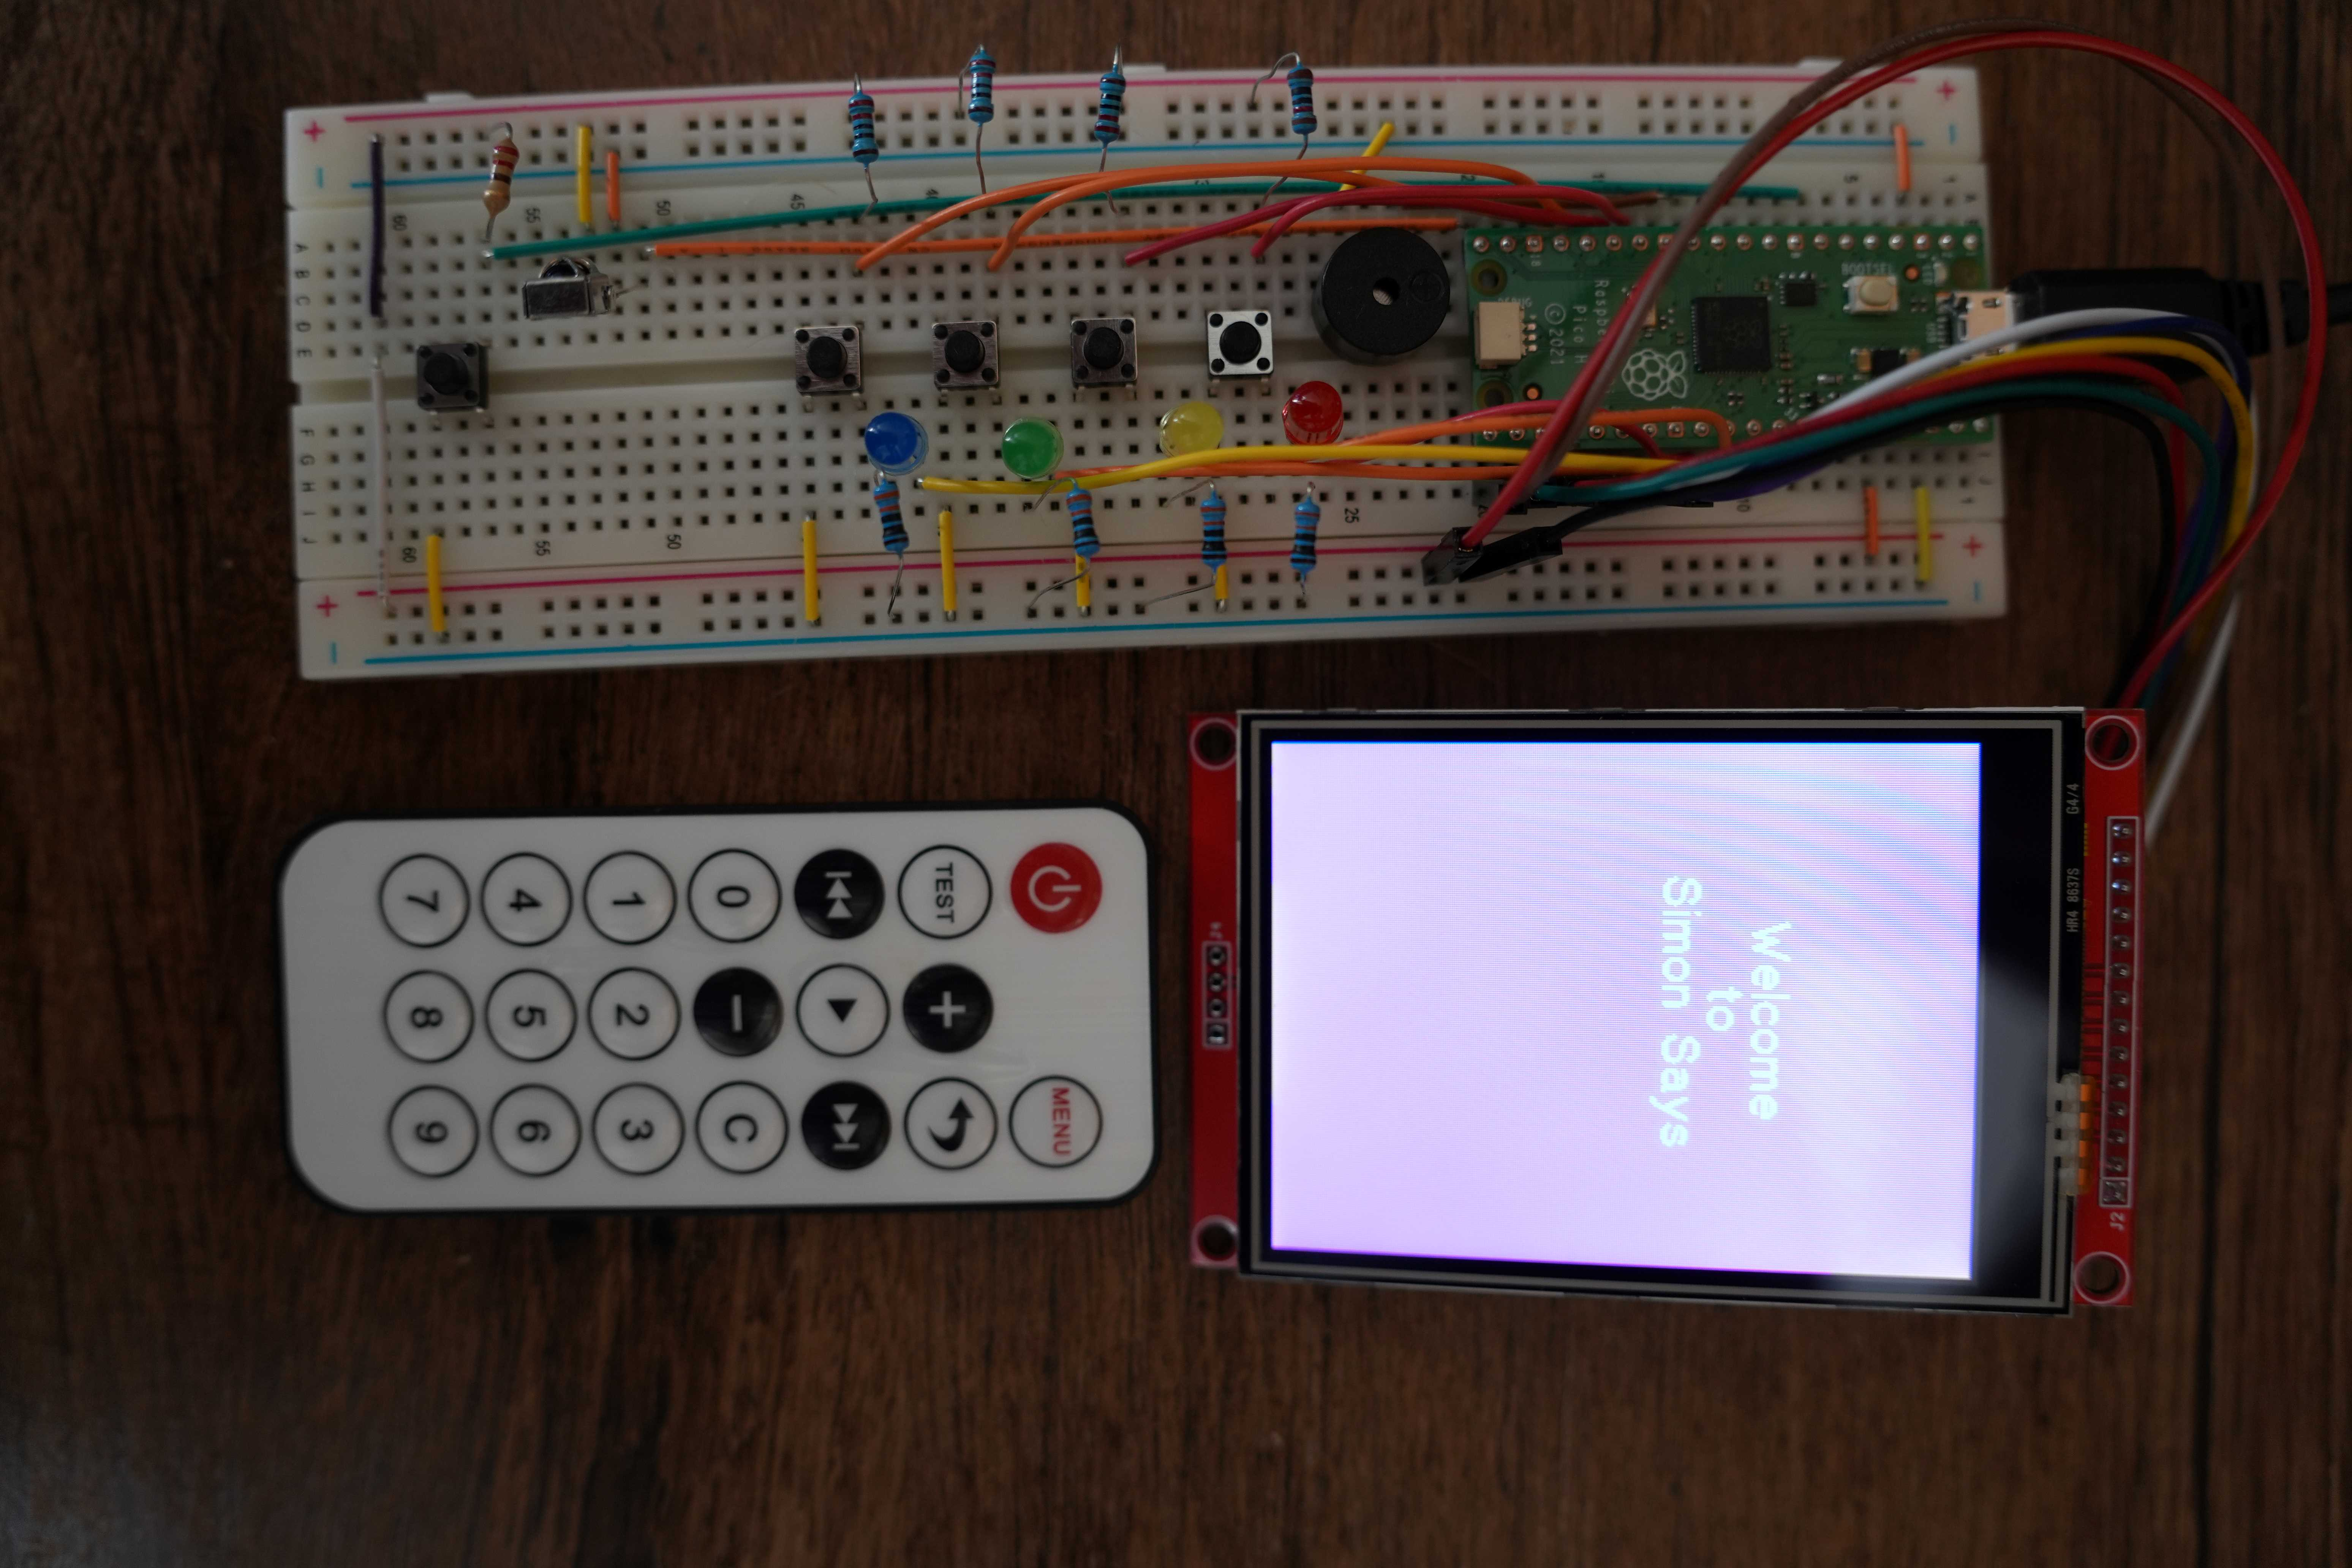
\includegraphics[width=\textwidth]{simon_says_compressed.jpg}
    \centering
    \caption{Hardware for Simon Says Game}
    \centering
    \label{fig:simon_says}
\end{figure}

Since no new assignments are being added to the class, the learning objectives for the 
class do not change.

\section{Recommendations for Course Integration}

does remember understand, apply and analyze. whole class is a progression

\section{Project Deliverables}

In the GitHub repository associated with this paper, which can be found in Appendix
\ref{appendix:appendix_github}, the folder titled ``6-computer-applications-in-me'' 
contains the rewritten lab assignment, code skeleton, and solution for the exercise
mentioned above. The folder also contains a README that details what is in each file
and what software is needed to complete the assignments. Installation instructions can
be found in the ``usage-and-installation'' folder in the GitHub repository.

The integration of these curriculum changes would not be a simple task. Since the 
entire class is structured around C++ and the ESP32, every lecture, assignment, quiz,
and test would have to be translated. In addition to this, new PCBs would need to be 
designed for use with the Pico. 

    
    \chapter{ME 571: Fluid Mechanics}
    \section{Course Overview}

ME 571: Fluid Mechanics is a lecture based class that focuses on the analysis
and kinematics of fluids through the application of the conservation equations, dimensional
analysis, and typical flow applications. The course is computation heavy and requires
a thorough understanding of the principles at play and the mathematics associated with them.
As such, fluid mechanics provides several opportunities to show the value of programming by
allowing students to focus on the principles at play rather than the advanced mathematics.

Due to the complexity of many problems in fluid mechanics, many software packages have been
created to relieve the computational burden from engineers. A few examples include:

\begin{itemize}
    \item System of Equation Solvers
    \begin{itemize}
        \item The most common of which is Engineering Equation Solver (EES), a 
        solver that contains a multitude of built-in functions 
        and properties for thermal and fluid sciences.
        \item Python and Excel also serve as capable equation solvers, though
        the experience is not nearly as tailored as EES.
    \end{itemize}
    \item Computational Fluid Dynamics (CFD)
    \begin{itemize}
        \item A CFD is a simulation program that uses numerical methods to solve fluid flow
        problems. They often output graphics, such as flow streamlines, that allow for
        a quick and easy analysis of the problem.
        \item Many popular CFD packages exist, such as ANSYS Fluent or SOLIDWORKS Flow Simulation.
    \end{itemize}
\end{itemize}

With software solutions being common in both industry and research, introducing students to
programmatic solution methods becomes even more important.

\section{New Assignment}

Currently, no assignments in ME 571: Fluid Mechanics make use of programming, but not for
the lack of options.
The study of fluid mechanics, as with many areas of engineering, requires the liberal 
application of differentials to solve problems and model systems. When given as
assignments, questions need to carefully crafted to ensure a symbolic solution can be found,
since finding a numerical solution is difficult and time-consuming. With the addition of
programming, however, finding a numerical solution becomes a trivial matter (assuming
standard numerical methods are appropriate for the problem).

Python has two libraries that excel at solving differentials, `sympy' for symbolic solutions 
and `scipy' for numerical solutions. The new assignment, Assignment \ref{fluid_assignment_1},
shows an example of using both sympy and scipy to solve a question that requires both
symbolic and numerical differentials. 

\assignments{ME 571: Assignment 1}
\label{fluid_assignment_1}

\begin{tcolorbox}[breakable, enhanced jigsaw, title=ME 571: Assignment \ref{fluid_assignment_1}, 
    colframe=ksu-purple, colback=ksu-gray]

    \textbf{Problem Statement}
    \parindent15pt

    As a valve is opened, water flows through the diffuser shown in Fig. P4.31 at an increasing 
    flow rate so that the velocity along the centerline is given by 
    $ \mathbf{V} = \it{u}\mathbf{\hat{i}}  = V_0(1 - \rm{e}^{-ct})(1 - \it{x/l})\mathbf{\hat{i}} $, 
    where $\it{u}$, $ \it{c} $, and $ \it{l} $ are constants. Determine the acceleration as 
    a function of $ \it{x} $ and $ \it{t} $. If $ V_0 = 10 ft/s $ and $ \it{l} = 5 $, what value 
    of $ \it{c} $ (other than $ \it{c} = 0 $) is needed to make the acceleration 0 for any 
    $ \it{x} $ at $ \it{t} = 1s $? Explain how the acceleration can be zero if the flow rate 
    is increasing with time? Be sure to leave specify all assumptions and comment on the 
    functionality of the code.

    \begin{center}
        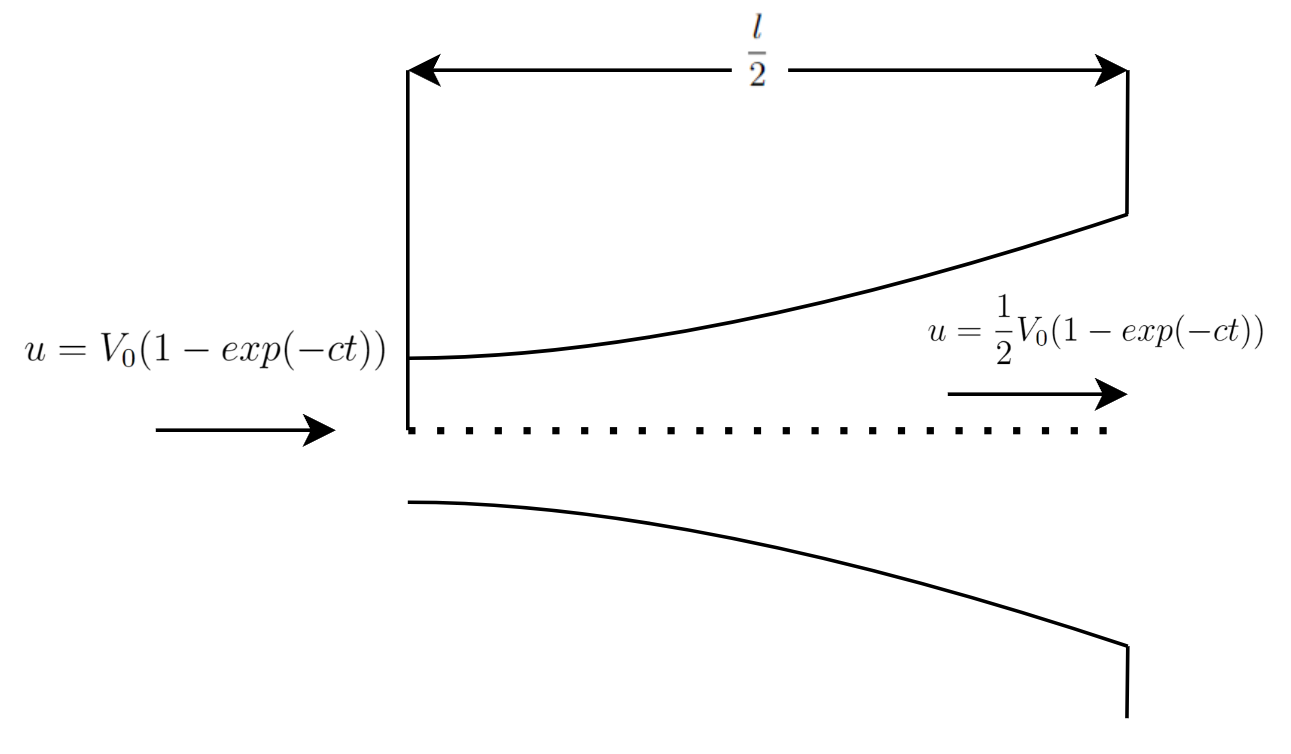
\includegraphics[width=\textwidth]{fluid-assignment1.png} 
    \end{center}

    \tcblower
    \textbf{Problem Solution}
    \parindent15pt

    For the full solution, see Appendix \ref{appendix:appendix_github}. Two solutions are 
    presented in the repository, and the entirety of solution 2 is shown below.

\begin{python}
from sympy import symbols, lambdify, diff, exp
from scipy.optimize import fsolve
from matplotlib import pyplot as plt
\end{python}

After importing the necessary libraries, we can set up the symbols that represent the 
constants and variables used in the equation. After that, create an equation for the 
velocity and use the `diff' function to get the acceleration equation.

\begin{python}
c, x, t, l, v = symbols("c x t l v")
vel = v*(1 - exp(-c * t))*(1 - x/l)
accel = diff(vel, t) + vel * diff(vel, x)
\end{python}

After getting the acceleration equation, we can substitute in the known values and then 
lambdify the equation, so we can use a numerical solver on it. Since the x-value does 
not matter for this equation, we can put in any value we want. We will opt for 1.

\begin{python}
accel = accel.subs({x: 1, t: 1, l: 5, v: 10})
acceleration = lambdify([c], accel, "scipy")
\end{python}

To use the fsolve function, you need to have an initial guess at the value. To get that
estimate, graph the acceleration function and observe where it crosses the x-axis.

\begin{python}
x = linspace(0, 1)
plt.hlines(0, 0, 1)
plt.plot(x, acceleration(x))
\end{python}

\begin{center}
    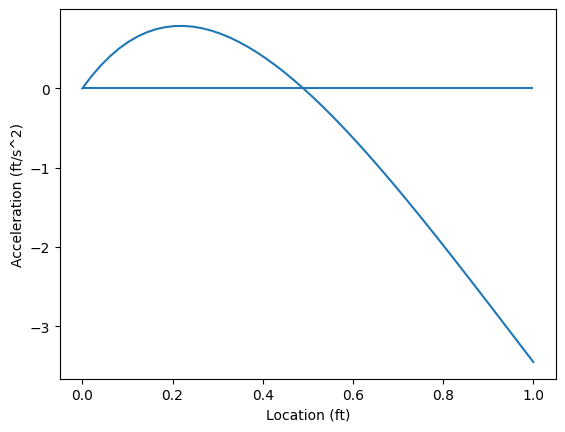
\includegraphics[scale=0.5]{fluid-plot.png}
\end{center}

Inspecting the graph shows an estimate value of 0.5. With that guess in hand, 
we can use fsolve to find the value.

\begin{python}
c = fsolve(acceleration, 0.5)
print(f"c = {c[0]:.4f} 1/s")
\end{python}

This gives an output of $ c = 0.491 \frac{1}{s} $.
\end{tcolorbox}

While the second solution is shown in Assignment \ref{fluid_assignment_1}, the first solution
assumes the student solved for the acceleration equation by hand and then used Python to
find the numerical solution.

\section{Project Deliverables}

In the GitHub repository associated with this paper, which can be found in 
Appendix \ref{appendix:appendix_github}, the folder titled ``7-fluid-mechanics''
contains both the problem statement and solution guide for the problem introduced in 
the previous section. The folder also contains a README that details what is in each file and 
what software is needed to complete the assignments. 

For these projects to be added to the class, the instructor would simply need to give the 
skeleton files to students as a problem statement. Given the use of specialized solving
methods used in the solution, an in-class example would be all but required.


    \chapter{ME 533: Machine Design}
    \section{Course Overview}

ME 533: Machine Design is a lecture based class that focuses on stress/strain analysis, load determination,
and failure theories. Despite being the first machine design class in the mechanical engineering curriculum, 
the material is a continuation of topics covered in two required civil engineering courses: CE 333: Statics
and CE 533: Mechanics of Materials.

As a higher level course that relies on well established theories and analysis methods, machine design
presents several opportunities for programmatic solutions to problems, though Excel calculators may
be more appropriate in some cases. Despite this, machine design does not require programming for 
assignments or projects, though this fact has varied depending on the current instructor. 

Homework assignments typically involve resolving loads on various members, analyzing the internal stresses, and 
determining the safety of a design using the appropriate failure theories. When appropriate, deformation
plots are drawn to highlight points of failure. The class finishes with discussions on spring and fastener
design, which involves heavy iteration.

\section{New Tool for Solving Assignments}

Since no assignments currently make use of programming, a new assignment with two questions have been solved 
to demonstrate potential uses for programming in the course. Rather than writing a Python script to solve 
iterative design or strictly numerical problems (see chapters on Thermodynamics, Fluid Mechanics, or 
Heat Transfer for examples of this), Assignment \ref{mach_des_assignment_1} focuses on finding and plotting 
beam deflection using singularity functions. 

\assignments{ME 533: Assignment 1}
\label{mach_des_assignment_1}

\begin{tcolorbox}[breakable, enhanced jigsaw, title=ME 533: Assignment \ref{mach_des_assignment_1}, 
    colframe=ksu-purple, colback=ksu-gray]

    \textbf{Problem Statement}
    \parindent15pt

    The following beam is subjected to the load shown. Determine the equation for deformation. 
    The beam is made of aluminum and has an I = 156 in\textsuperscript{4}. Assume EI is constant. Graph 
    the shear, moment, slope, and deflection.

    \begin{center}
        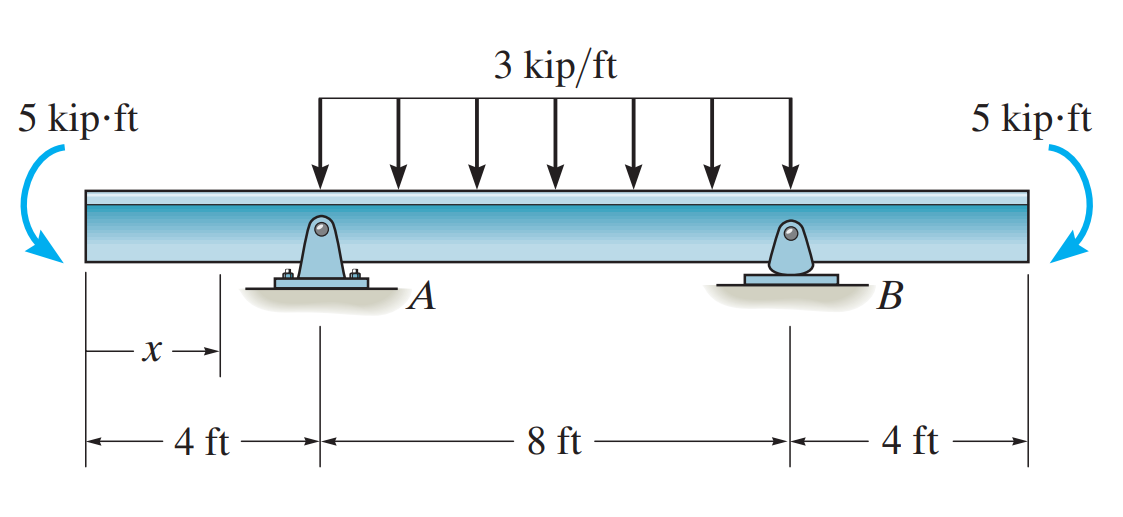
\includegraphics[width=\textwidth]{mach-des-assingment1.png}
    \end{center}

    \tcblower
    \textbf{Problem Solution}
    \parindent15pt

    For the full solution, see Appendix \ref{appendix:appendix_github}. The following code shows how to
    launch the Singularity Solver from a Jupyter Notebook.

\begin{python}
import subprocess

output = subprocess.run(
    ["python", "-m", "singularity"], 
    shell=True, 
    capture_output=True,
    cwd="./MNE/machine_design"
)
print(output.stdout.decode("ascii"))
\end{python}

After inputting the beam attributes, loading state, and boundary conditions, the following graph
is produced.

\begin{center}
    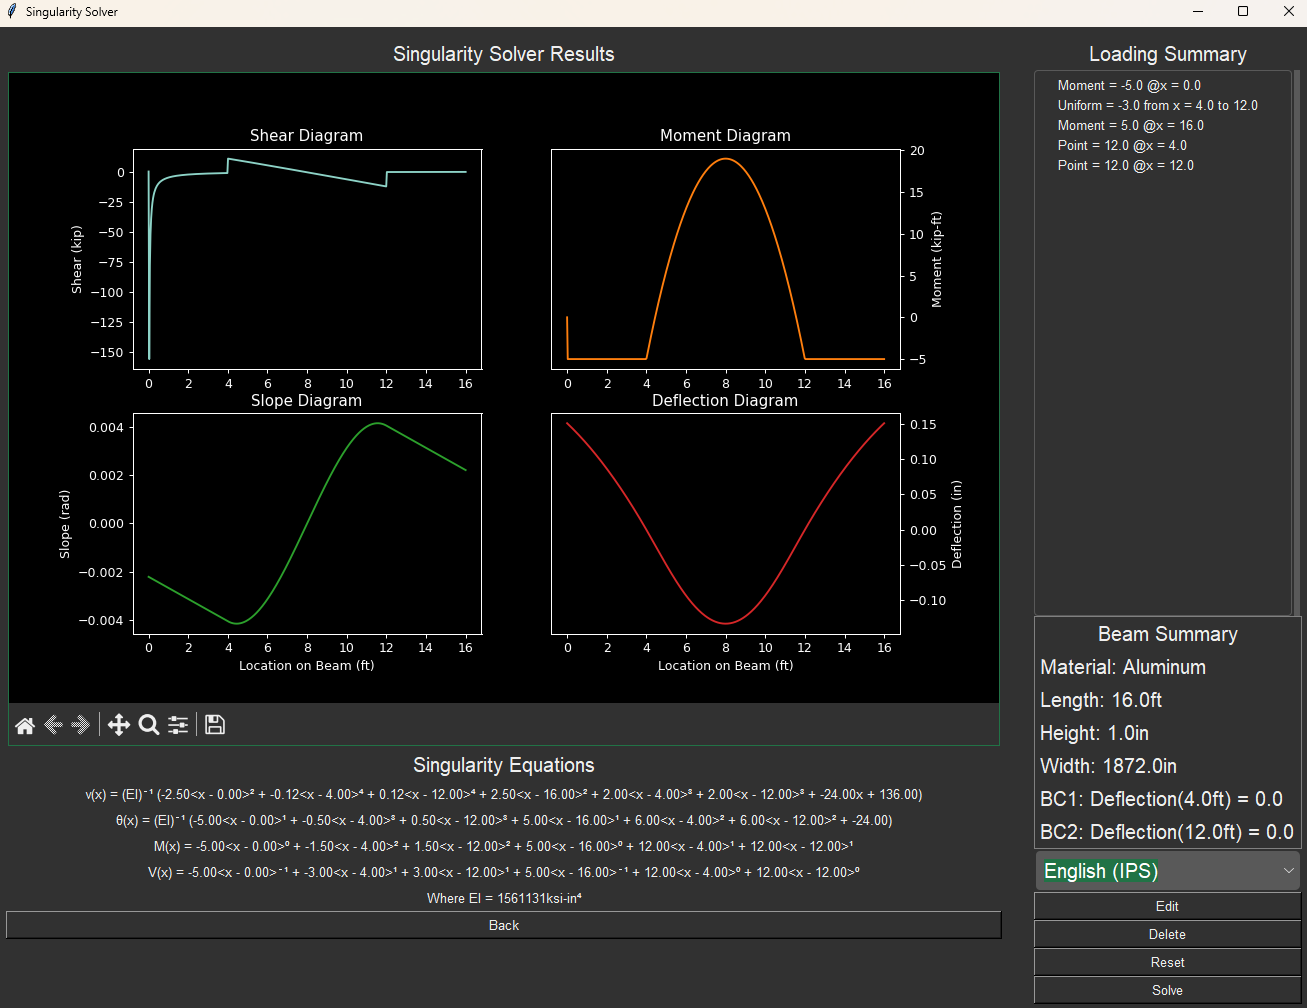
\includegraphics[width=\textwidth]{mach-des-graph.png}
\end{center}
\end{tcolorbox}

\begin{figure}[h]
    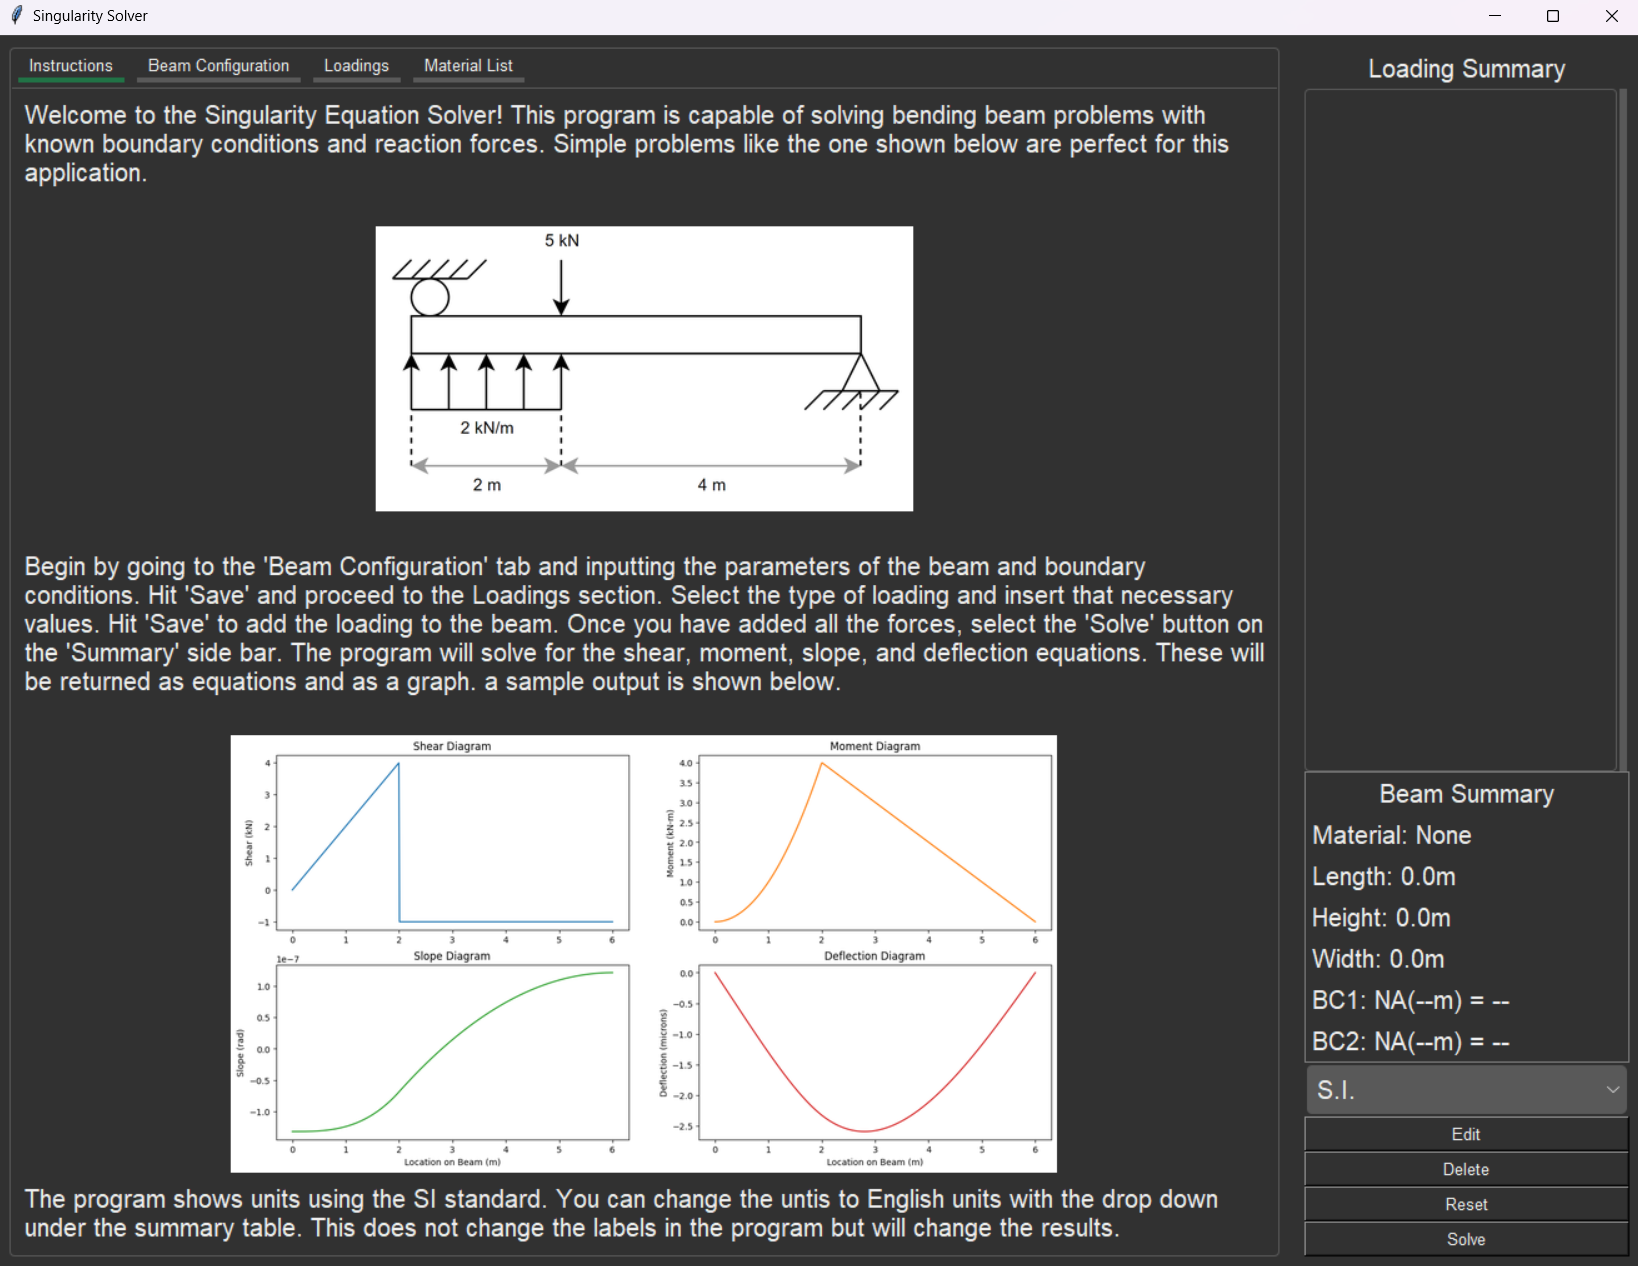
\includegraphics[width=\textwidth]{singularity-gui.png}
    \centering
    \caption{Singularity Solver GUI}
    \centering
    \label{fig:singularity-gui}
\end{figure}

The most simple adoption of programming into singularity function assignments would be requiring computer
generated plots. Students would first solve for reaction forces, create a singularity equation, integrate
several times, and then create a plot using the deformation equation. The solution presented here takes a 
higher level approach by accepting the loading forces on the bar and then creating and integrating the 
singularity equation automatically. This is done through a graphical user interface developed and executed
in Python.

The GUI can be launched in Python (Assignment \ref{mach_des_assignment_1}) or through
the terminal as a Python module. Once launched, the application will open in a new window, which is shown
in Figure \ref{fig:singularity-gui}. The home page contains instructions for using the solver, so the details 
here will be sparing. The second page is dedicated to beam configuration, including length, cross-section, 
material, and boundary conditions. The next page presents various forms of loading to add
to the beam. The last page allows custom materials to be added to the list of materials.

While the GUI currently automates significant portions of singularity problems, several features should be
added at a later date, including non-rectangular cross-sections (though a workaround is presented) and
the ability to add supports to the beam. This would give the program the ability to calculate the reaction
forces and determine boundary conditions without relying on the user to correctly find and input them.

Since this application takes most of the work out of the hands of the students, it would not be a good tool
for teaching singularity functions. Rather, the application would be best utilized when finding the shear,
moment, slope, or deformation of a beam is one part in the context of a larger problem. Additionally, 
it would serve as a realistic look at how most analysis is done in industry - by a computer.

Using programming in this manner gives students a better idea of how real problems are solved by
introducing them to a more efficient and powerful solution method. These questions would also 
directly correlate to Abet Student Outcomes 1, 6, and 7, as seen in Appendix 
\ref{appendix:appendix_abet} and weekly correlates to Outcome 3.

\section{Project Deliverables}

In the GitHub repository associated with this paper, which can be found in Appendix \ref{appendix:appendix_github},
the folder titled ``8-machine-design'' contains both the problem statements and solution guides for the two questions
introduced in the previous section. The folder also contains a README that details what is in each file and 
what software is needed to complete the assignments. 

For these projects to be added to the class, the instructor would  need to give the skeleton files to 
students as a problem statement and the MNE folder as Python library. Using one of the two questions as an in-class
example would serve as a good opportunity to remind students how to use Python with Jupyter Notebooks and to 
demonstrate how to open and use the singularity function GUI.


    \chapter{ME 570: Control of Mechanical Systems I}
    \section{Course Overview}

ME 570: Control of Mechanical Systems is a mixed class with two lectures and one lab every week. The lectures focus on teaching
the principles and theory of controls while the lab focuses on designing and testing control systems. Most labs are dedicated to
using and designing PID controllers using different methods, such as frequency analysis or pole analysis.

To complete the labs, the class makes use of a custom motor rig called a motorlab, show in Figure \ref{fig:motorlab}. To go 
along with the motorlab, a graphical user interface for controlling the motorlab was also created by Dale Schinstock, also 
shown in Figure \ref{fig:motorlab}. This GUI runs as an application through MATLAB and allows the students to both send 
commands to the motor and collect runtime data from the motor.

\begin{figure}
    \centering
    \begin{subfigure}{.5\textwidth}
      \centering
      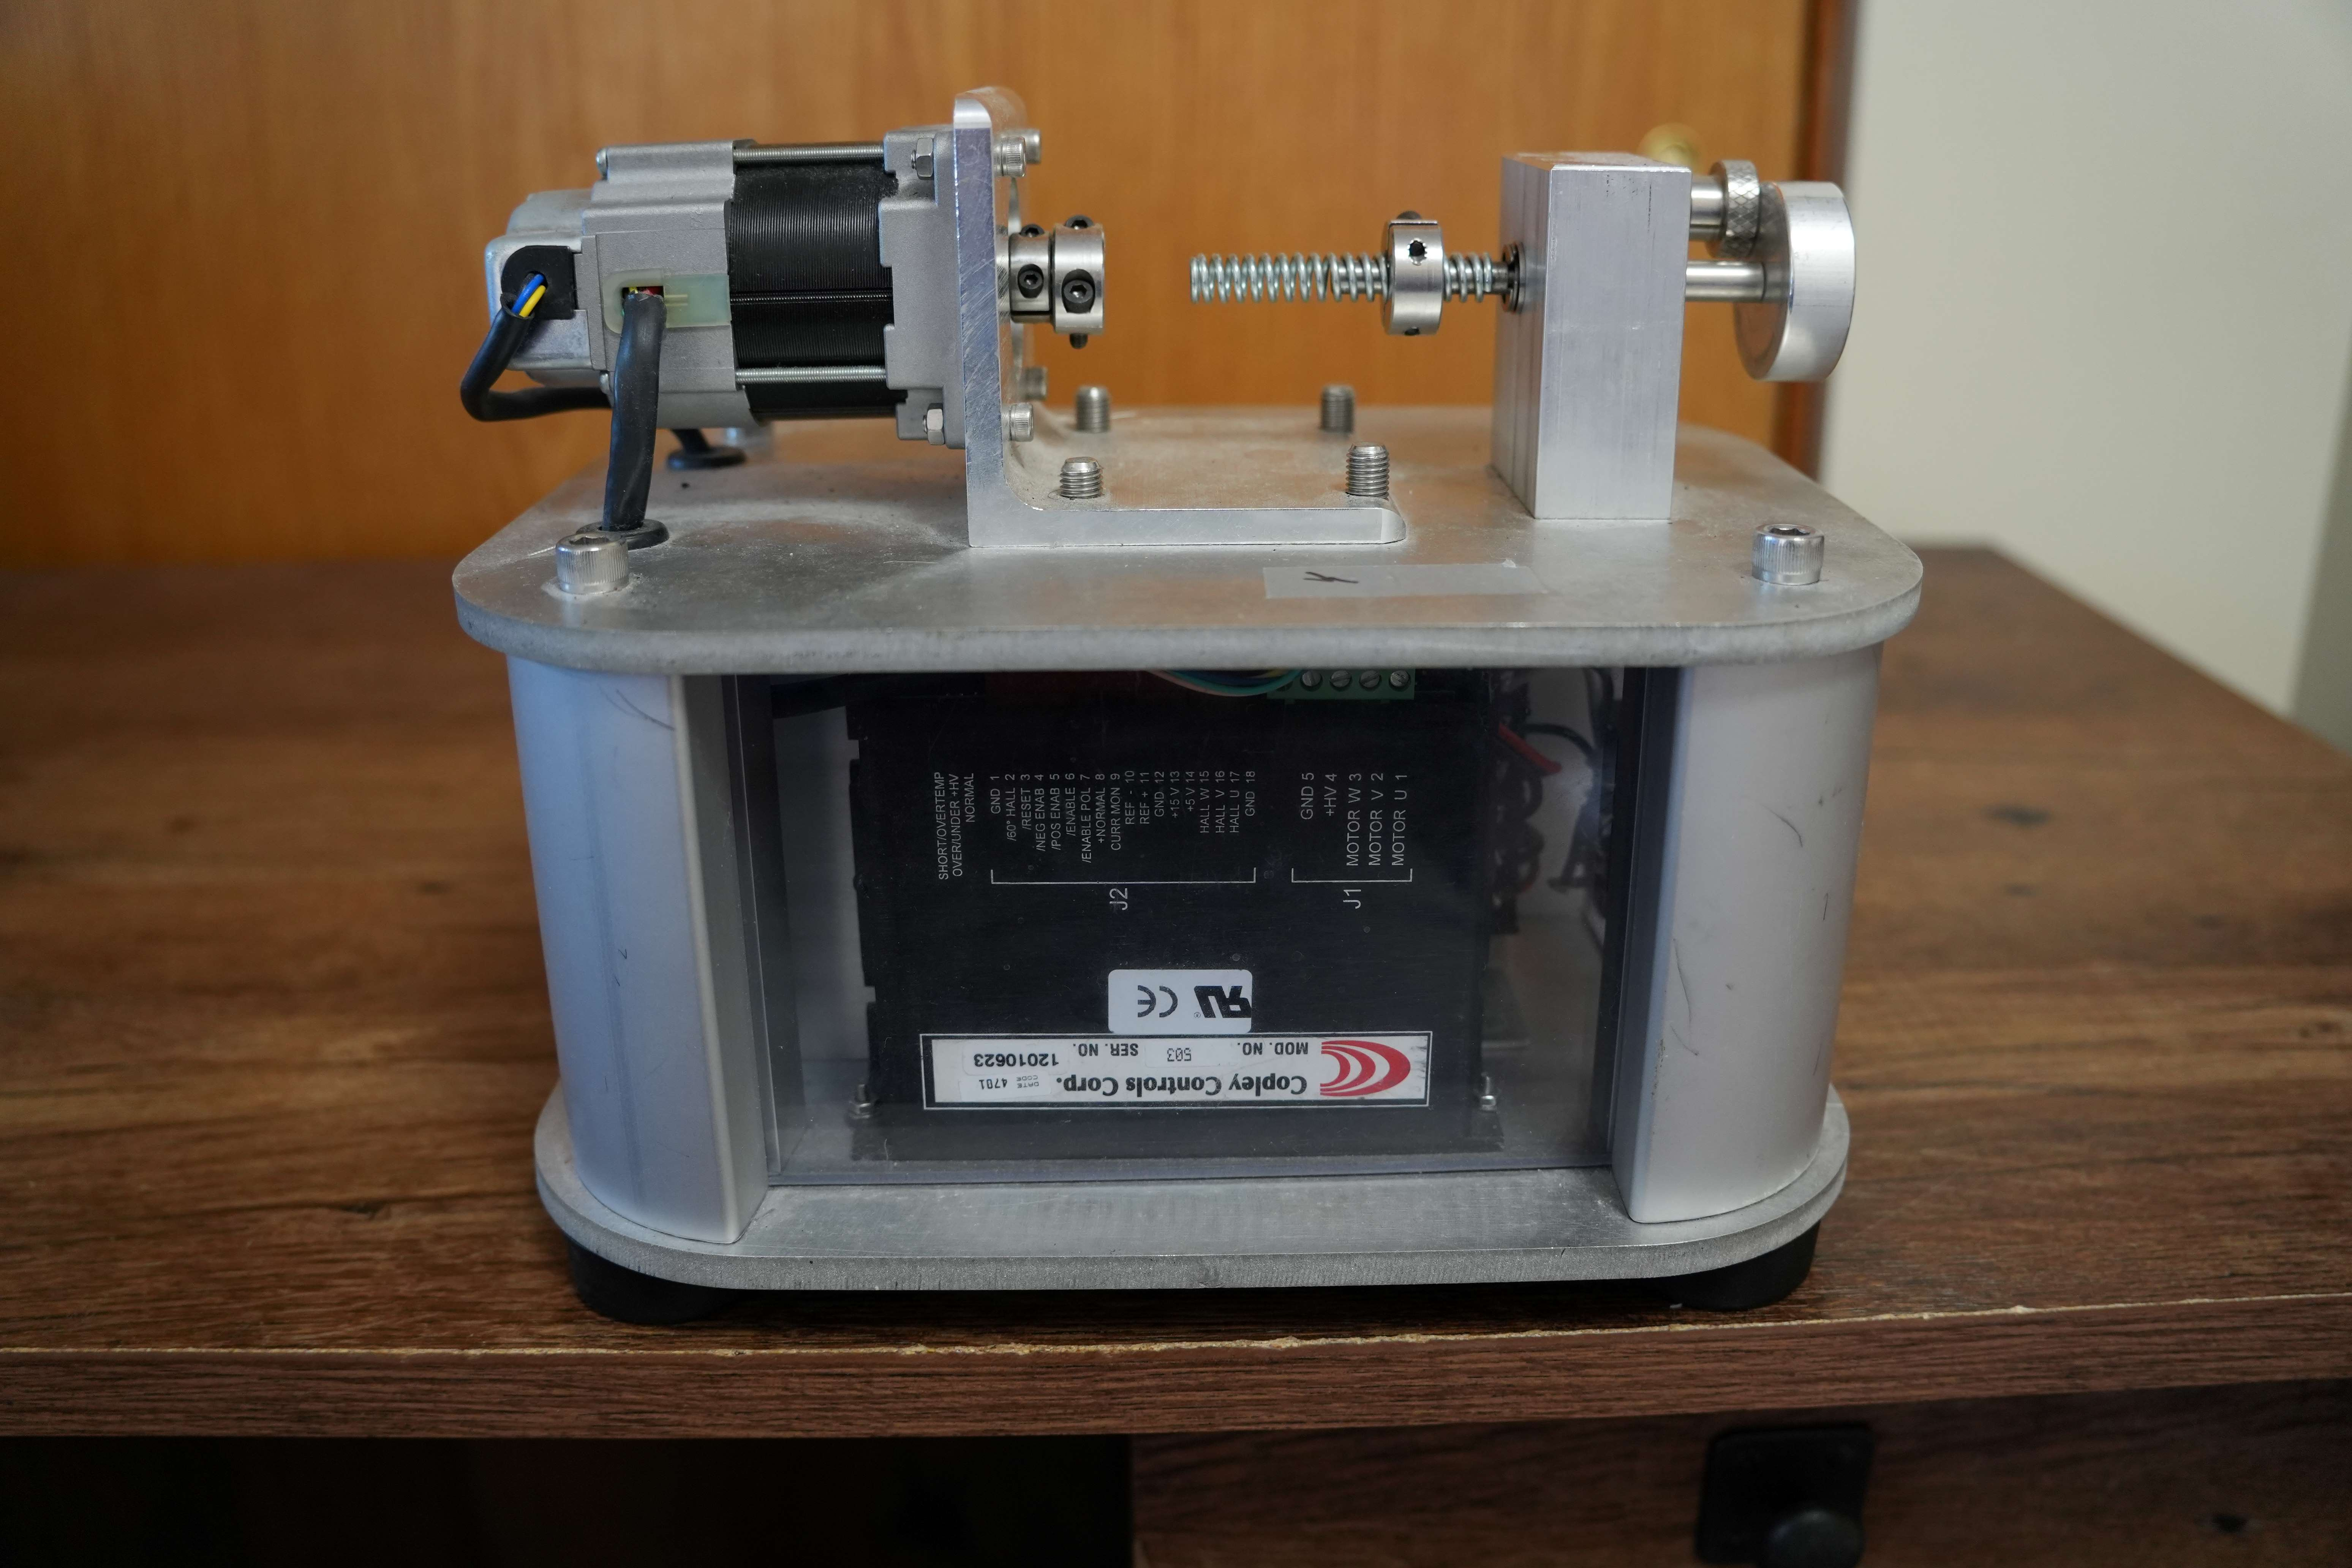
\includegraphics[width=\linewidth]{motorlab.jpg}
      \caption{The motorlab apparatus}
      \label{fig:motorlab-device}
    \end{subfigure}%
    \begin{subfigure}{.5\textwidth}
      \centering
      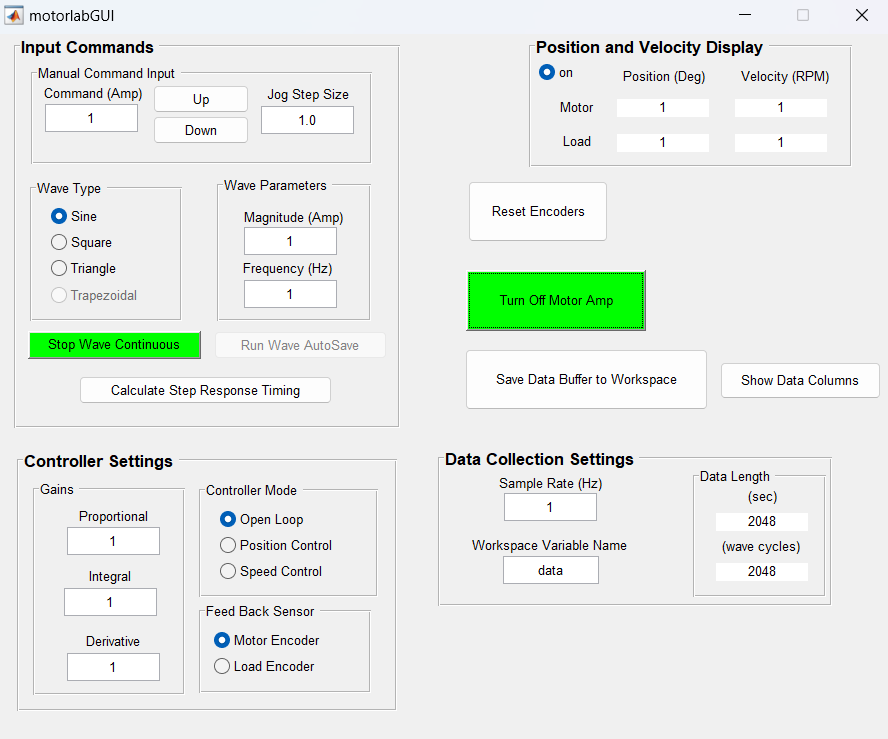
\includegraphics[width=0.8\linewidth]{motorlabgui.png}
      \caption{The motorlabGUI interface}
      \label{fig:motorlabgui}
    \end{subfigure}
    \caption{The motorlab system designed by Dale Schinstock}
    \label{fig:motorlab}
\end{figure}

Controls also relies heavily on MATLAB for the completion of lab and homework assignments. All work is done using .mlx files through a 
licensed copy of MATLAB for a more interactive working environment. To access the controls related commands, a package called 
the Controls Toolbox has to be purchased from MATLAB. 

While Controls uses programming more than any class besides ME 400, little to no instruction is provided on how to program in MATLAB.
The first lab is dedicated to taking the MATLAB Onramp starter course, which takes about 1 to 2 hours to complete. However, the 
Onramp does not address most of the work done in Controls, such as plotting and transfer functions. The Onramp does teach students
the basics of MATLAB syntax, but most students come out of the Onramp just as confused by MATLAB as they were going in.

This disconnect between students and MATLAB becomes a barrier that prevents students from understanding controls. Many students
spend more time trying to understand MATLAB than they do learning controls. 

\section{Lab Assignment Redesigns}

Since ME 570 already fully utilizes programming in the course, no new assignments are being created. Instead, three pre-existing
labs have been translated from MATLAB to Python. While MATLAB is the industry standard when it comes to control systems, the
license is expensive, students do not have a solid understanding of it, and we do not make use of its most powerful feature,
Simulink. In addition to this, a third-party Python library, aptly named $control$, has a MATLAB module that imitates the Control
Toolbox, both in form and functionality, from MATLAB. In combination with Jupyter Notebooks and a few custom plotting modifications,
using Python will give a very similar experience to MATLAB, and will give students that pursue the field of controls any easy
transition to MATLAB. 

All three translated labs make use of the motorlab, which has had its GUI turned into an application, courtesy of the MATLAB
Compiler. This allows the application to be run from an app icon or from the terminal. These labs also make use of a custom plot
command. The plot command builds on the standard $matplotlib$ \cite{Hunter_Matplotlib_A_2D_2007} plot command and adds the ability to 
create data tips. A right mouse click will add a data tip at the click location, and a double left click in the plot window 
will remove all data tips. More custom functions could be added later to imitate MATLAB functionality as needed, but this was the 
only one required for completing these labs.

The first translated lab, Lab 4, is a standard controls assignment that makes use of the motorlab, reading the csv output from the
motorlab, and plotting the results \cite{controls-4}. 

\assignments{ME 570: Assignment 1}
\label{control_assignment_1}

\begin{tcolorbox}[breakable, enhanced jigsaw, title=ME 570: Assignment \ref{control_assignment_1}, 
    colframe=ksu-purple, colback=ksu-gray]

    \textbf{Problem Statement}
    \parindent15pt

    For the full problem statement, please see Appendix \ref{appendix:appendix_github}. Estimate
    the damping ratio by fitting an envelope to the step response.
    
    \tcblower
    \textbf{Problem Solution}
    \parindent15pt

    For the full solution, see Appendix \ref{appendix:appendix_github}. The solution shown below
    highlights the use of data from the motorlabGUI and plotting with custom data tips.

    To achieve an environment similar to MATLAB, the following imports are required at the top of the file.

\begin{python}
%matplotlib widget
from matplotlib.pyplot import figure, xlabel, ylabel, legend, show, title, xlim, ylim
from custom_functions import plot
from control.matlab import tf, step
from numpy import polyfit, array
from math import pi, sqrt
from pandas import read_csv
\end{python}

\begin{python}
J = 1.1e-5 + 0.19e-5
ks = k_estimate
Kdc = kt/ks
wn = sqrt(ks / J)
zeta_estimate = 0.05
 
# Generate a step response from a first order system 
# with a pole equal to the real part of the
# 2nd order poles
real_part = zeta_estimate * wn
envelope_TF = tf(Kdc * real_part, [1, real_part])
[envelope_y, envelope_time] = step(envelope_TF)
\end{python}

The following code assumes that the motorlabGUI data was collected
and saved with the name ``stepdata.csv.'' Here, `read\_csv' and
`iloc' from the $pandas$ library are used for clean file reading.

\begin{python}
# Extract data from the generated step response
stepdata = read_csv("stepdata.csv", header=None)

# extract time column of the data matrix
dataTime = stepdata.iloc[:,0]

# extract third angle column of the data matrix
dataAngle = stepdata.iloc[:,2]

# convert to rad
dataTh = kdr * dataAngle
\end{python}

After the data has been loaded into the workbook, a graph of the step
response can be plotted.

\begin{python}
plot(dataTime, dataTh, envelope_time, envelope_y, '--')
ylabel('Angular Position (rad)')
xlabel('Time (sec)')
ylim(-0.01, 0.55)
xlim(-0.01, 0.7)
title('Step Response Data with Estimated Envelope')
legend(['step response from Motorlab','estimated envelope'])
show()
\end{python}

\begin{center}
    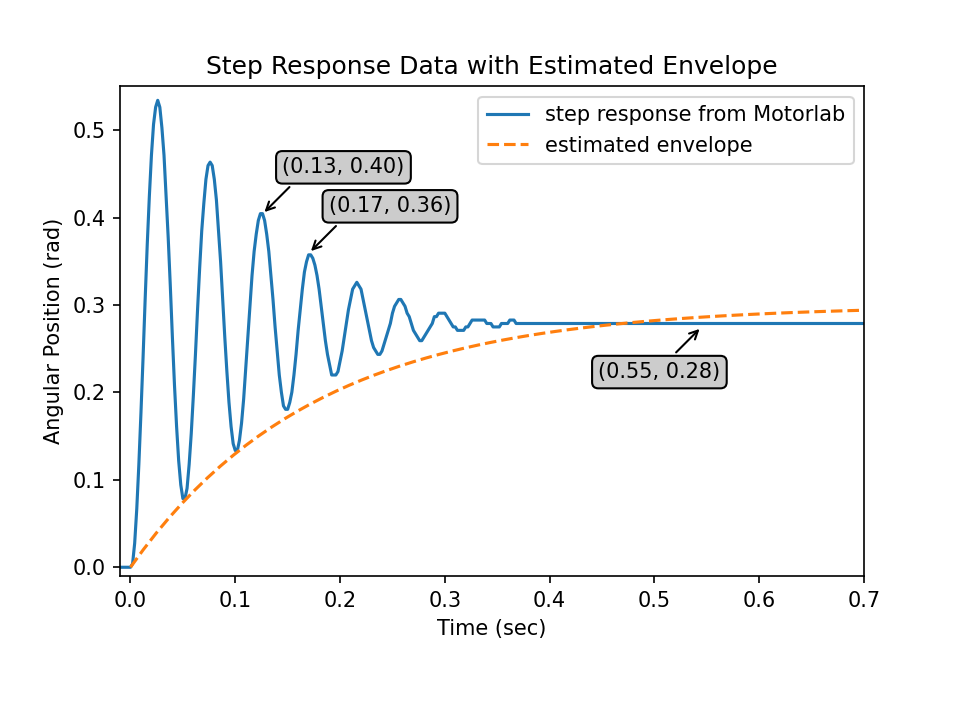
\includegraphics[width=\textwidth]{controls-assignment1-graph.png}
\end{center}

\end{tcolorbox}

The second lab, Lab 10 \cite{controls-10}, builds on Lab 4 by adding root locus plots through 
a tool called sisotool. Sisotool outputs four interactive plots that allow the user to move pole 
locations to see how the system responds. While the sisotool command in Python is not as powerful 
as the full designer in MATLAB, it does provide the full functionality used in ME 570.

\assignments{ME 570: Assignment 2}
\label{control_assignment_2}

\begin{tcolorbox}[breakable, enhanced jigsaw, title=ME 570: Assignment \ref{control_assignment_2}, 
    colframe=ksu-purple, colback=ksu-gray]

    \textbf{Problem Statement}
    \parindent15pt

    For the full problem statement, please see Appendix \ref{appendix:appendix_github}. Create a
    controller for the motorlab and plot the poles using sisotool.
    
    \tcblower
    \textbf{Problem Solution}
    \parindent15pt

    For the full solution, see Appendix \ref{appendix:appendix_github}. Below is an example of 
    setting up a transfer function and a controller and then using sisotool to analyze the system.

\begin{python}
b = 3e-5
kdr = 180/pi
J = 1.29e-5
kt = 0.05

s = tf('s')
Gm= kt*kdr / (J*s**2+b*s)
Gc2 = 10*.00007 + .00007*s
\end{python}

After the transfer function and controller have been made, sisotool can be used to adjust the poles.

\begin{python}
figure()
sisotool(Gc2*Gm)
show()
\end{python}

Grabbing and moving the black squares will allow the user to move the pole locations.

\begin{center}
    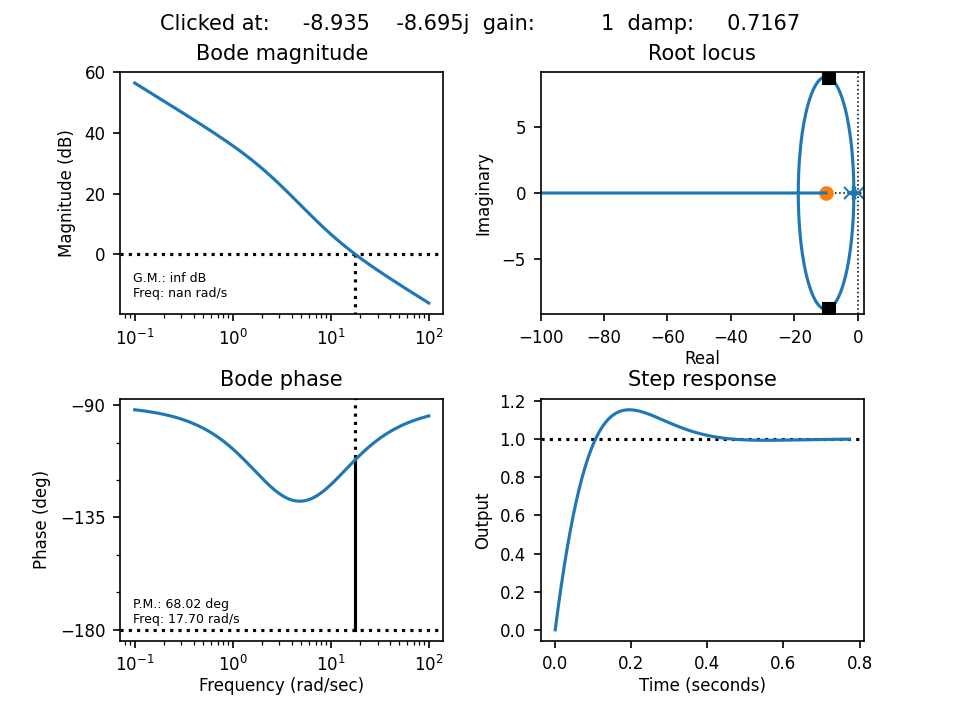
\includegraphics[width=\textwidth]{controls-assignment2-sisotool.png}
\end{center}
\end{tcolorbox}

The third lab, Lab 13, focuses on frequency response design methods and utilizes Bode plots \cite{controls-13}.

\assignments{ME 570: Assignment 3}
\label{control_assignment_3}

\begin{tcolorbox}[breakable, enhanced jigsaw, title=ME 570: Assignment \ref{control_assignment_3}, 
    colframe=ksu-purple, colback=ksu-gray]

    \textbf{Problem Statement}
    \parindent15pt

    For the full problem statement, please see Appendix \ref{appendix:appendix_github}. Given the 
    natural frequency and DC gain derived from the table (not shown here), construct a new transfer 
    function, that will hopefully better match the data.
    
    \tcblower
    \textbf{Problem Solution}
    \parindent15pt

    For the full solution, see Appendix \ref{appendix:appendix_github}. The following code is an
    example of using Bode in Python to do frequency analysis.

\begin{python}
wn = 19.18*2*pi # natural freq from data (rad/s)
Kdc = 23 # dc gain from data in deg/Amp
Mwn = 540 # magnitude ratio at wn from data in deg/Amp
zeta = Kdc/Mwn/2 # calc damp ratio using Mwn and Kdc
Gnew = (Kdc*wn**2) / (s**2 + 2*zeta*wn*s + wn**2)

mnew, pnew, wnew = bode(Gnew) # get mag, phase, freq
mnew = 20 * log10(mnew)
pnew = (180 / pi) * pnew # Convert radians to degrees
\end{python}

With the new data models complete, graph them using a logarithmic plot.

\begin{python}
figure()
subplot(2, 1, 1)
semilogx(wnew, mnew, w, m, wdata, magdata, '*')
title('Bode Plot')
ylabel('magnitude (dB)')
xlabel('freq (rad/s)')

subplot(2, 1, 2); 
semilogx(wnew, pnew, w, p, wdata, phdata, '*')
ylabel('phase (deg)');
xlabel('freq (rad/s)')
legend(['improved', 'original', 'data'])
show()
\end{python}

\begin{center}
    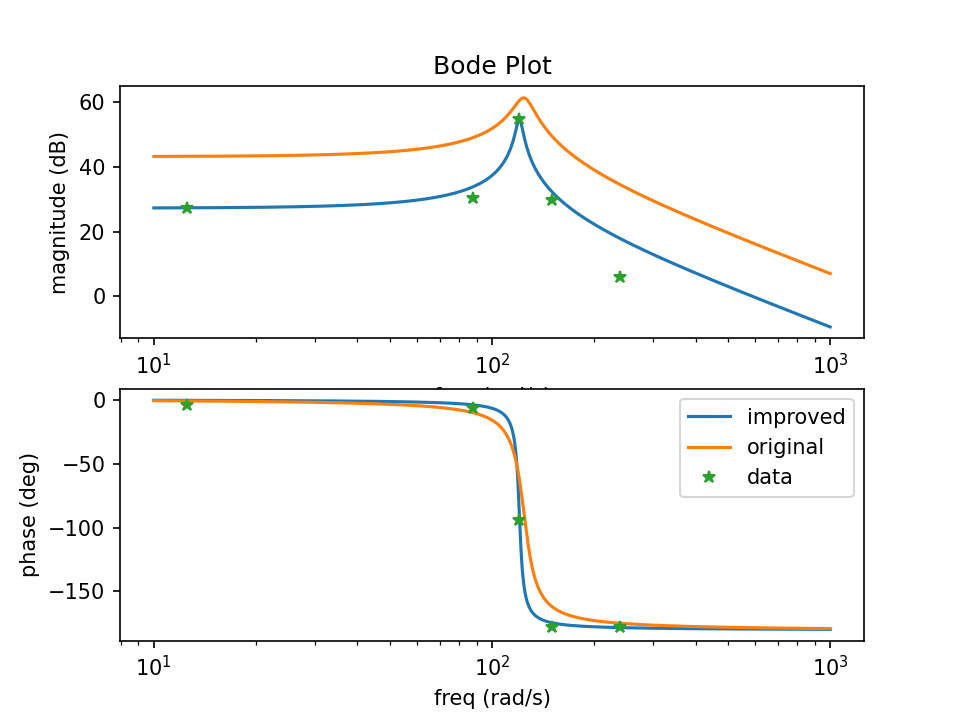
\includegraphics[width=\textwidth]{controls-assignment3-bode.png}
\end{center}
\end{tcolorbox}

The labs chosen aim to showcase how the major features used in MATLAB can be emulated in Python. Some features, like Simulink, have
no direct correlation. However, Simulink is only used in one lab, and students only need to make two small changes. Python also
requires more library imports, but these can all be handled by the starting code and do not pose much concern.

Since no new assignments are being added to the class, the learning objectives for the class do not change.

\section{Recommendations for Course Integration}

After completing ME 570, students should be able to organize code in a structured manner, critique the functionality of written
code, and produce high quality code for the purpose of modeling a control system. 

Since no new assignments are being added to the class, only one change is recommended outside the adoption of a new language.
As the semester progresses, students should be given fewer and fewer lines of starting code, with a greater burden being placed
on the students to generate their own solutions. During the lab practical, students should be expected to work from scratch,
organizing and writing their own program. This gradual removal of the training wheels will be the final step in teaching 
students how to program in the required curriculum.

\section{Project Deliverables}

In the GitHub repository associated with this paper, which can be found in Appendix \ref{appendix:appendix_github},
the folder titled ``9-control-of-mechanical-systems'' contains the lab assignments, starting code files, and solutions for the three
lab assignments explained above. The folder also contains a README that details what is in each file and what software is needed 
to complete the assignments. 

The act of integrating these labs into the class would not be as simple as the integrations for other classes. Since every lab 
uses MATLAB, the other 11 labs would also need to be translated. In addition to this, every computer in the lab would need to 
get the correct applications, extensions, and motorlabGUI executable installed. Instructions for installing everything needed 
can be found in the ``usage-and-installation'' folder in the GitHub repository.


    \chapter{ME 573: Heat Transfer}
    \section{Course Overview}

ME 573: Heat Transfer is lecture based class that focuses on analyzing systems using
the three modes of heat transfer: conduction, convection, and radiation. The study of
heat transfer is dense with equations, analysis methods, and tables, most of which
provide opportunities for programming to be used for solving problems, whether that
be Excel calculators or Python. Of these, perhaps the most practical application 
is the design of heat exchangers. Accordingly, the only project in the class is an 
iterative heat exchanger design problem, which requires the use of Excel or Python.

\section{Project Modifications}

Since a project that makes use of programming already exists for Heat Transfer, no
changes have been made to the assignment. The problem statement can be found unchanged
in the heat-transfer repository as well as a solution made using Python in a Jupyter
Notebook.

In lieu of changing the project itself, additional resource were made to mimic the 
functionality of an MNE Python library. The library contains methods for getting 
the properties of water and oil needed to complete the project. Rather than saving
large tables of data, fourth order polynomials were fit to the data using 
`scipy.optimize.curve\_fit' to allow for a smaller package size. The purpose-built
library also has a function for the Reynolds number. 

While this library currently contains exactly what is needed to complete the project,
the end-of-the-line goal is a library that contains every property and equation that
could be needed.

Since no new assignments or requirements are being added, the learning objectives
for the class do not change. 

\section{Project Deliverables}

In the GitHub repository associated with this paper, which can be found in 
Appendix \ref{appendix:appendix_github}, the folder titled ``10-heat-trasnfer''
contains both the problem statement and solution guide for the project introduced in 
the previous section. The folder also contains a README that details what is in each file and 
what software is needed to complete the assignments. 

For these projects to be added to the class, the instructor would simply need to give the 
skeleton files to students as a problem statement. It may be beneficial to give students 
an example of how to use the look-up methods in the MNE library. 

    
    \chapter{Conclusion and Future Work}
    \section{Concerns}
Something about all hardware used and all software packages used? 
That might be more appropriate somewhere else?

Future work includes creation of libraries that have all the table 
data from text books. Some exist already, but not all of them. Might 
be better to have an in-house collection.

\section{Recommendations}


    \appendix
    \chapter{Project Repository}
    \label{appendix:appendix_github}
    https://github.com/mKiloLA/python-based-mne

    \chapter{Software Versions}
    \label{appendix:appendix_versions}
    Through the entirity of this paper, the following application, package, and extension versions are used:

\begin{itemize}
    \item Applications
    \begin{itemize}
        \item Python 3.12.0
            \begin{itemize}
                \item Optionally, Python 3.11.5 through Anaconda 2023.09
            \end{itemize}
        \item Visual Studio Code 1.85
    \end{itemize}
    \item Python Packages
    \begin{itemize}
        \item control v0.9.4
        \item ipykernel v6.27.1
        \item ipympl v0.9.3
        \item matplotlib v3.8.2
        \item mendeleev v0.15.0
        \item numpy v1.26.2
        \item pandas v2.1.4
        \item physdata v0.2.0
        \item PYroMat v2.2.4
        \item pyXSteam v0.4.9
        \item scipy v1.11.4
        \item sympy v1.12
    \end{itemize}
    \item Visual Studio Code Extensions
    \begin{itemize}
        \item Python v2023.22.1
        \item Pylance v2023.12.1
        \item MicroPico v3.5.0
        \item Jupyter v2023.11.1003402403
        \item Jupyter Keymap v1.1.2
        \item Jupyter Notebook Renderers v1.0.17 
        \item Jupyter Cell Tags v0.1.8
        \item Jupyter Slide Show v0.1.5
        \item IntelliCode v1.2.30
        \item IntelliCode API Usage Examples v0.2.8
        \item vscode-pdf v1.2.2
        \item Excel Viewer v4.2.58
    \end{itemize}
\end{itemize}

    \chapter{Abet Student Outcomes}
    \label{appendix:appendix_abet}
    The following excerpt is taken directly from K-State's website \cite{abet}:

Student outcomes describe what students are expected to know and be 
able to do by the time of graduation. These relate to the knowledge, 
skills and behaviors that students acquire as they progress through 
the program. The mechanical engineering program will enable students 
to attain the following, by the time of graduation:
\begin{enumerate}
    \item an ability to identify, formulate, and solve complex engineering problems by applying principles of engineering, science, and mathematics
    \item an ability to apply engineering design to produce solutions that meet specified needs with consideration of public health, safety, and welfare, as well as global, cultural, social, environmental, and economic factors
    \item an ability to communicate effectively with a range of audiences
    \item an ability to recognize ethical and professional responsibilities in engineering situations and make informed judgments, which must consider the impact of engineering solutions in global, economic, environmental, and societal contexts
    \item an ability to function effectively on a team whose members together provide leadership, create a collaborative and inclusive environment, establish goals, plan tasks, and meet objectives
    \item an ability to develop and conduct appropriate experimentation, analyze and interpret data, and use engineering judgment to draw conclusions
    \item an ability to acquire and apply new knowledge as needed, using appropriate learning strategies.
\end{enumerate}

https://www.mne.k-state.edu/academics/accreditation/


    
\end{document}
